
\documentclass[frontgrid, backgrid,a4,12pt]{flacards}
\usepackage{color}
\usepackage{graphicx}
\usepackage{etoolbox}
\pretocmd{\card}{\def\curhint{}}{}{}

\pagesetup{2}{4}

% Chinese support
\usepackage{xeCJK}

\renewcommand{\cardtextstylef}{\Huge}
\renewcommand{\cardtextstyleb}{\small}
\renewcommand{\brfoot}{}
\renewcommand{\bcfoot}{\let\\\relax\footnotesize\curhint}
\renewcommand{\flhead}{\footnotesize\thecardno}
\renewcommand{\brhead}{\footnotesize\thecardno}

\usepackage{array}
\usepackage{multirow}
\usepackage{ragged2e}

\newcommand{\inputfield}{\rule[-1mm]{3cm}{0.5pt}}
\begin{document}
\card{\centering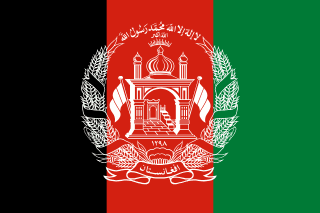
\includegraphics[width=0.3\textwidth]{flags/af.png}}{
\begin{tabular}{m{3cm} m{5cm}} \textbf{Afganistan} & \textbf{阿富汗} \\[0.5em] \multicolumn{1}{m{3cm}}{\raggedright Kabul\\喀布尔\\Pashto / Dari\\普什图语 / 达里语} &
\raggedright \textbf{Fact:} La cometa es un símbolo cultural en Afganistán? Hay competencias tradicionales de corte de cometas… ¡como batallas aéreas con hilo!
\end{tabular}
}
\card{\centering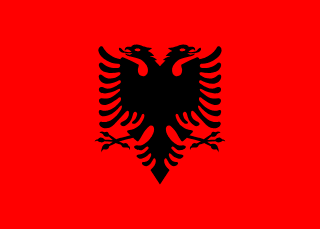
\includegraphics[width=0.3\textwidth]{flags/al.png}}{
\begin{tabular}{m{3cm} m{5cm}} \textbf{Albania} & \textbf{阿尔巴尼亚} \\[0.5em] \multicolumn{1}{m{3cm}}{\raggedright Tirana\\地拉那\\Albanian\\阿尔巴尼亚语} &
\raggedright \textbf{Fact:} En Albania al mover la cabeza, asienten para decir no y niegan para decir sí. ¡Puede causar confusión entre extranjeros!
\end{tabular}
}
\card{\centering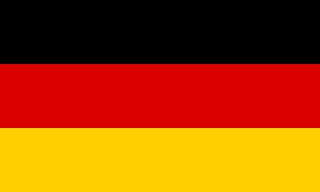
\includegraphics[width=0.3\textwidth]{flags/de.png}}{
\begin{tabular}{m{3cm} m{5cm}} \textbf{Germany} & \textbf{德国} \\[0.5em] \multicolumn{1}{m{3cm}}{\raggedright Berlin\\柏林\\German\\德语} &
\raggedright \textbf{Fact:} En Alemania puedes tener una carrera profesional como catador oficial de cerveza? Se llama Bier-Sommelier.
\end{tabular}
}
\card{\centering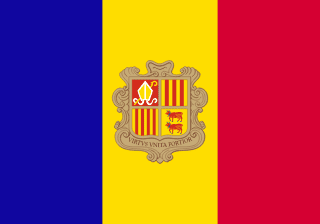
\includegraphics[width=0.3\textwidth]{flags/ad.png}}{
\begin{tabular}{m{3cm} m{5cm}} \textbf{Andorra} & \textbf{安道尔} \\[0.5em] \multicolumn{1}{m{3cm}}{\raggedright Andorra la Vella\\安道尔城\\Catalan\\加泰罗尼亚语} &
\raggedright \textbf{Fact:} Andorra no tiene ejército propio y solo tiene dos jefes de Estado: ¡el presidente de Francia y un obispo de España!
\end{tabular}
}
\card{\centering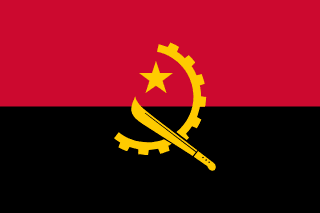
\includegraphics[width=0.3\textwidth]{flags/ao.png}}{
\begin{tabular}{m{3cm} m{5cm}} \textbf{Angola} & \textbf{安哥拉} \\[0.5em] \multicolumn{1}{m{3cm}}{\raggedright Luanda\\罗安达\\Portuguese\\葡萄牙语} &
\raggedright \textbf{Fact:} En Angola los peinados tradicionales no son solo moda. Algunos indican estado civil, edad o incluso tribu.
\end{tabular}
}
\card{\centering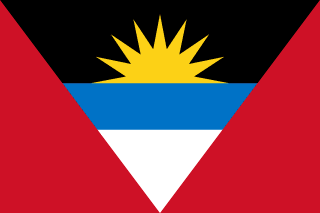
\includegraphics[width=0.3\textwidth]{flags/ag.png}}{
\begin{tabular}{m{3cm} m{5cm}} \textbf{Antigua and Barbuda} & \textbf{安提瓜和巴布达} \\[0.5em] \multicolumn{1}{m{3cm}}{\raggedright Saint John’s\\圣约翰\\English\\英语} &
\raggedright \textbf{Fact:} Este país tiene más playas que días del año. ¡Una por cada día y aún te sobran!
\end{tabular}
}
\card{\centering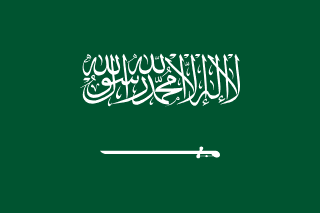
\includegraphics[width=0.3\textwidth]{flags/sa.png}}{
\begin{tabular}{m{3cm} m{5cm}} \textbf{Saudi Arabia} & \textbf{沙特阿拉伯} \\[0.5em] \multicolumn{1}{m{3cm}}{\raggedright Riyadh\\利雅得\\Arabic\\阿拉伯语} &
\raggedright \textbf{Fact:} En Arabia Saudita hay una ciudad futurista planeada para ser 170 km en línea recta, sin autos ni calles Se llama NEOM.
\end{tabular}
}
\card{\centering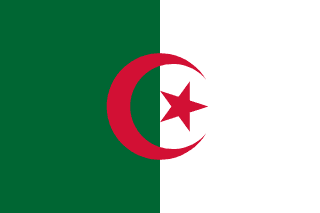
\includegraphics[width=0.3\textwidth]{flags/dz.png}}{
\begin{tabular}{m{3cm} m{5cm}} \textbf{Algeria} & \textbf{阿尔及利亚} \\[0.5em] \multicolumn{1}{m{3cm}}{\raggedright Algiers\\阿尔及尔\\Arabic / Berber\\阿拉伯语 / 柏柏尔语} &
\raggedright \textbf{Fact:} El Sahara cubre más del 80\% de Argelia ¡Pero aún así tienen pistas de esquí en sus montañas del norte!
\end{tabular}
}
\card{\centering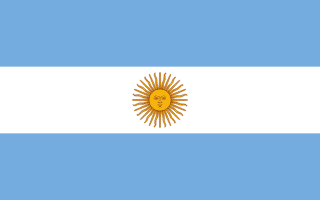
\includegraphics[width=0.3\textwidth]{flags/ar.png}}{
\begin{tabular}{m{3cm} m{5cm}} \textbf{Argentina} & \textbf{阿根廷} \\[0.5em] \multicolumn{1}{m{3cm}}{\raggedright Buenos Aires\\布宜诺斯艾利斯\\Spanish\\西班牙语} &
\raggedright \textbf{Fact:} En Argentina el 20 de julio se celebra el Día del Amigo y hasta los desconocidos se saludan ¡Es como un San Valentín de la amistad!
\end{tabular}
}
\card{\centering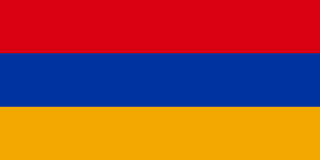
\includegraphics[width=0.3\textwidth]{flags/am.png}}{
\begin{tabular}{m{3cm} m{5cm}} \textbf{Armenia} & \textbf{亚美尼亚} \\[0.5em] \multicolumn{1}{m{3cm}}{\raggedright Yerevan\\埃里温\\Armenian\\亚美尼亚语} &
\raggedright \textbf{Fact:} Armenia fue el primer país en adoptar el cristianismo como religión oficial en el año 301 d.C. ¡Antes que el Imperio Romano!
\end{tabular}
}
\card{\centering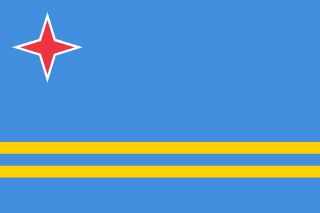
\includegraphics[width=0.3\textwidth]{flags/aw.png}}{
\begin{tabular}{m{3cm} m{5cm}} \textbf{Aruba} & \textbf{阿鲁巴} \\[0.5em] \multicolumn{1}{m{3cm}}{\raggedright Oranjestad\\奥拉涅斯塔德\\Dutch / Papiamento\\荷兰语 / 帕皮阿门托语} &
\raggedright \textbf{Fact:} En Aruba los postes de luz están pintados con rayas para que los turistas no los confundan con árboles
\end{tabular}
}
\card{\centering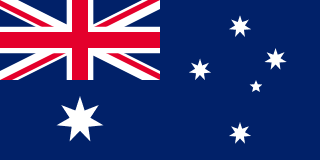
\includegraphics[width=0.3\textwidth]{flags/au.png}}{
\begin{tabular}{m{3cm} m{5cm}} \textbf{Australia} & \textbf{澳大利亚} \\[0.5em] \multicolumn{1}{m{3cm}}{\raggedright Canberra\\堪培拉\\English\\英语} &
\raggedright \textbf{Fact:} En Australia hay más canguros que personas ¡Y algunos pueblos tienen señales de tránsito con canguros cruzando!
\end{tabular}
}
\card{\centering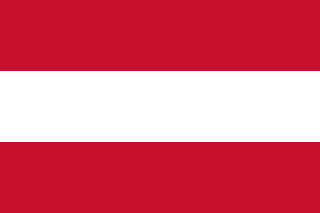
\includegraphics[width=0.3\textwidth]{flags/at.png}}{
\begin{tabular}{m{3cm} m{5cm}} \textbf{Austria} & \textbf{奥地利} \\[0.5em] \multicolumn{1}{m{3cm}}{\raggedright Vienna\\维也纳\\German\\德语} &
\raggedright \textbf{Fact:} En Austria hay una biblioteca de abejas. Cada “libro” es una colmena con registros de comportamiento y genética.
\end{tabular}
}
\card{\centering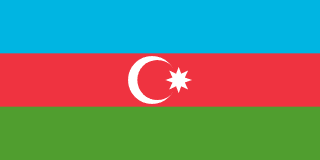
\includegraphics[width=0.3\textwidth]{flags/az.png}}{
\begin{tabular}{m{3cm} m{5cm}} \textbf{Azerbaijan} & \textbf{阿塞拜疆} \\[0.5em] \multicolumn{1}{m{3cm}}{\raggedright Baku\\巴库\\Azerbaijani\\阿塞拜疆语} &
\raggedright \textbf{Fact:} En Azerbaiyán hay volcanes que “escupen” lodo en lugar de lava ¡Y hacen ruidos como si el planeta tuviera gases!
\end{tabular}
}
\card{\centering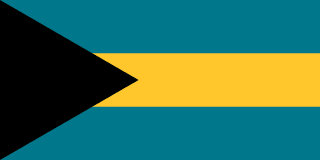
\includegraphics[width=0.3\textwidth]{flags/bs.png}}{
\begin{tabular}{m{3cm} m{5cm}} \textbf{Bahamas} & \textbf{巴哈马} \\[0.5em] \multicolumn{1}{m{3cm}}{\raggedright Nassau\\纳苏\\English\\英语} &
\raggedright \textbf{Fact:} En las Bahamas hay un agujero azul tan profundo que podría tragarse la Torre Eiffel. ¡Se llama Dean’s Blue Hole!
\end{tabular}
}
\card{\centering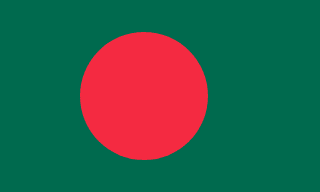
\includegraphics[width=0.3\textwidth]{flags/bd.png}}{
\begin{tabular}{m{3cm} m{5cm}} \textbf{Bangladesh} & \textbf{孟加拉国} \\[0.5em] \multicolumn{1}{m{3cm}}{\raggedright Dhaka\\达卡\\Bengali\\孟加拉语} &
\raggedright \textbf{Fact:} En Bangladés hay un tren tan lleno que muchos viajan en el techo? ¡Parece una escena de película de acción!
\end{tabular}
}
\card{\centering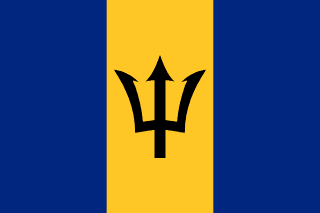
\includegraphics[width=0.3\textwidth]{flags/bb.png}}{
\begin{tabular}{m{3cm} m{5cm}} \textbf{Barbados} & \textbf{巴巴多斯} \\[0.5em] \multicolumn{1}{m{3cm}}{\raggedright Bridgetown\\布里奇敦\\English\\英语} &
\raggedright \textbf{Fact:} Barbados tiene una cueva subterránea con su propio tranvía turístico. ¡Una montaña rusa natural llamada Harrison's Cave!
\end{tabular}
}
\card{\centering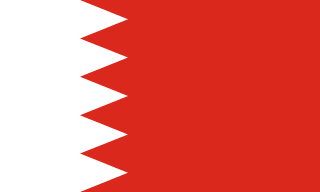
\includegraphics[width=0.3\textwidth]{flags/bh.png}}{
\begin{tabular}{m{3cm} m{5cm}} \textbf{Bahrain} & \textbf{巴林} \\[0.5em] \multicolumn{1}{m{3cm}}{\raggedright Manama\\马纳马\\Arabic\\阿拉伯语} &
\raggedright \textbf{Fact:} En el medio del desierto de Baréin crece un árbol solitario desde hace más de 400 años, sin fuente de agua visible?
\end{tabular}
}
\card{\centering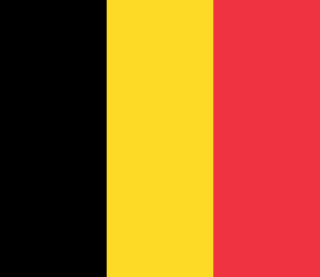
\includegraphics[width=0.3\textwidth]{flags/be.png}}{
\begin{tabular}{m{3cm} m{5cm}} \textbf{Belgium} & \textbf{比利时} \\[0.5em] \multicolumn{1}{m{3cm}}{\raggedright Brussels\\布鲁塞尔\\Dutch / French / German\\荷兰语 / 法语 / 德语} &
\raggedright \textbf{Fact:} Bélgica tiene más castillos por kilómetro cuadrado que cualquier otro país del mundo. ¡Una tierra de cuentos!
\end{tabular}
}
\card{\centering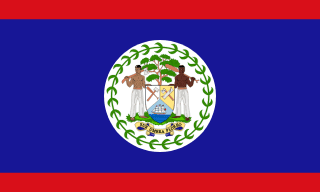
\includegraphics[width=0.3\textwidth]{flags/bz.png}}{
\begin{tabular}{m{3cm} m{5cm}} \textbf{Belize} & \textbf{伯利兹} \\[0.5em] \multicolumn{1}{m{3cm}}{\raggedright Belmopan\\贝尔莫潘\\English\\英语} &
\raggedright \textbf{Fact:} Belice tiene la segunda barrera de coral más grande del mundo, hogar de tiburones que parecen sonreír.
\end{tabular}
}
\card{\centering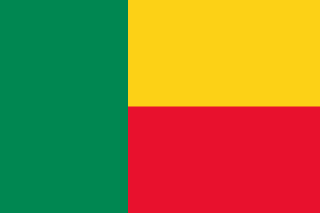
\includegraphics[width=0.3\textwidth]{flags/bj.png}}{
\begin{tabular}{m{3cm} m{5cm}} \textbf{Benin} & \textbf{贝宁} \\[0.5em] \multicolumn{1}{m{3cm}}{\raggedright Porto-Novo\\波尔图诺伏\\French\\法语} &
\raggedright \textbf{Fact:} El vudú nació en Benín y es una religión oficial. ¡Sí, con festivales y todo!
\end{tabular}
}
\card{\centering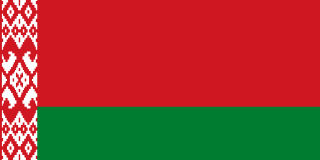
\includegraphics[width=0.3\textwidth]{flags/by.png}}{
\begin{tabular}{m{3cm} m{5cm}} \textbf{Belarus} & \textbf{白俄罗斯} \\[0.5em] \multicolumn{1}{m{3cm}}{\raggedright Minsk\\明斯克\\Belarusian / Russian\\白俄罗斯语 / 俄语} &
\raggedright \textbf{Fact:} Bielorrusia es uno de los pocos países donde el KGB todavía existe y se llama exactamente así.
\end{tabular}
}
\card{\centering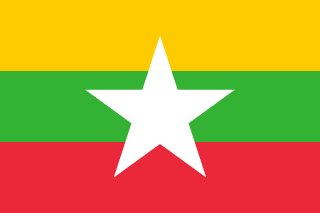
\includegraphics[width=0.3\textwidth]{flags/mm.png}}{
\begin{tabular}{m{3cm} m{5cm}} \textbf{Myanmar} & \textbf{缅甸} \\[0.5em] \multicolumn{1}{m{3cm}}{\raggedright Naypyidaw\\内比都\\Burmese\\缅甸语} &
\raggedright \textbf{Fact:} En Birmania el calendario tradicional tiene 8 días a la semana. ¡El miércoles está dividido en dos!
\end{tabular}
}
\card{\centering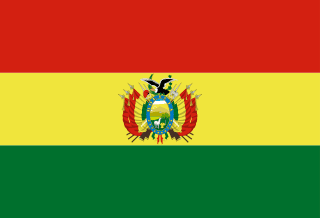
\includegraphics[width=0.3\textwidth]{flags/bo.png}}{
\begin{tabular}{m{3cm} m{5cm}} \textbf{Bolivia} & \textbf{玻利维亚} \\[0.5em] \multicolumn{1}{m{3cm}}{\raggedright Sucre / La Paz \\苏克雷 / 拉巴斯\\Spanish\\西班牙语} &
\raggedright \textbf{Fact:} Bolivia tiene una “autopista” blanca de sal tan grande que parece un espejo del cielo? Es el Salar de Uyuni.
\end{tabular}
}
\card{\centering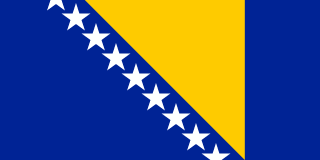
\includegraphics[width=0.3\textwidth]{flags/ba.png}}{
\begin{tabular}{m{3cm} m{5cm}} \textbf{Bosnia and Herzegovina} & \textbf{波斯尼亚和黑塞哥维那} \\[0.5em] \multicolumn{1}{m{3cm}}{\raggedright Sarajevo\\萨拉热窝\\Bosnian\\波斯尼亚语} &
\raggedright \textbf{Fact:} En Bosnia hay una pirámide más alta que las de Egipto. Según algunos, ¡de origen desconocido!
\end{tabular}
}
\card{\centering
\includegraphics[width=0.3\textwidth]{flags/bw.png}}{
\begin{tabular}{m{3cm} m{5cm}} \textbf{Botswana} & \textbf{博茨瓦纳} \\[0.5em] \multicolumn{1}{m{3cm}}{\raggedright Gaborone\\哈博罗内\\English / Setswana\\英语 / 塞茨瓦纳语} &
\raggedright \textbf{Fact:} Botsuana alberga una población de elefantes tan grande que hay señales de tráfico especiales para ellos.
\end{tabular}
}
\card{\centering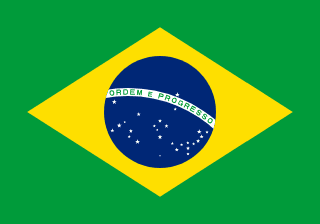
\includegraphics[width=0.3\textwidth]{flags/br.png}}{
\begin{tabular}{m{3cm} m{5cm}} \textbf{Brazil} & \textbf{巴西} \\[0.5em] \multicolumn{1}{m{3cm}}{\raggedright Brasilia\\巴西利亚\\Portuguese\\葡萄牙语} &
\raggedright \textbf{Fact:} En Brasil hay un festival llamado la guerra de frutas. Es en Parintins y combina danza, teatro y frutas voladoras.
\end{tabular}
}
\card{\centering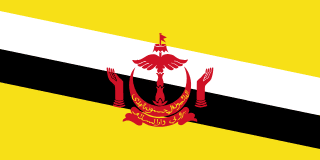
\includegraphics[width=0.3\textwidth]{flags/bn.png}}{
\begin{tabular}{m{3cm} m{5cm}} \textbf{Brunei} & \textbf{文莱} \\[0.5em] \multicolumn{1}{m{3cm}}{\raggedright Bandar Seri Begawan\\斯里巴加湾市\\Malay\\马来语} &
\raggedright \textbf{Fact:} En Brunéi el sultán tiene su propio avión Boeing 747… ¡con grifos de oro en el baño!
\end{tabular}
}
\card{\centering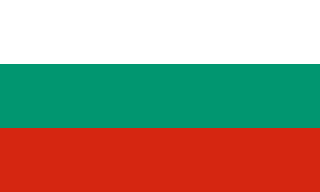
\includegraphics[width=0.3\textwidth]{flags/bg.png}}{
\begin{tabular}{m{3cm} m{5cm}} \textbf{Bulgaria} & \textbf{保加利亚} \\[0.5em] \multicolumn{1}{m{3cm}}{\raggedright Sofia\\索非亚\\Bulgarian\\保加利亚语} &
\raggedright \textbf{Fact:} En Bulgaria se considera de mala suerte regalar flores en número par. ¡Solo impares, por favor!
\end{tabular}
}
\card{\centering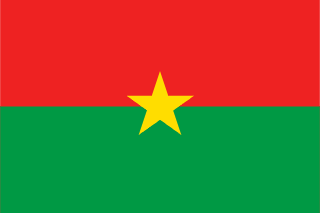
\includegraphics[width=0.3\textwidth]{flags/bf.png}}{
\begin{tabular}{m{3cm} m{5cm}} \textbf{Burkina Faso} & \textbf{布基纳法索} \\[0.5em] \multicolumn{1}{m{3cm}}{\raggedright Ouagadougou\\瓦加杜古\\French\\法语} &
\raggedright \textbf{Fact:} En Burkina Faso existe un cine al aire libre que funciona con energía solar en medio del desierto. ¡Cine ecológico bajo las estrellas!
\end{tabular}
}
\card{\centering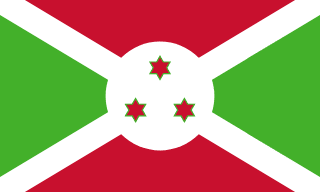
\includegraphics[width=0.3\textwidth]{flags/bi.png}}{
\begin{tabular}{m{3cm} m{5cm}} \textbf{Burundi} & \textbf{布隆迪} \\[0.5em] \multicolumn{1}{m{3cm}}{\raggedright Gitega\\基特加\\Kirundi\\基鲁恩迪语} &
\raggedright \textbf{Fact:} Burundi tiene su propia “ceremonia del tambor” tan importante que fue declarada Patrimonio de la Humanidad por la UNESCO?
\end{tabular}
}
\card{\centering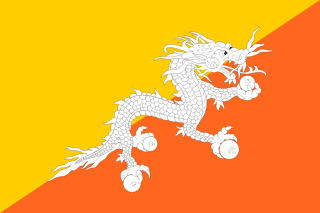
\includegraphics[width=0.3\textwidth]{flags/bt.png}}{
\begin{tabular}{m{3cm} m{5cm}} \textbf{Bhutan} & \textbf{不丹} \\[0.5em] \multicolumn{1}{m{3cm}}{\raggedright Thimphu\\廷布\\Dzongkha\\宗卡语} &
\raggedright \textbf{Fact:} En Bután se mide el bienestar nacional con un Índice de Felicidad Bruta. ¡La felicidad es más importante que el dinero!
\end{tabular}
}
\card{\centering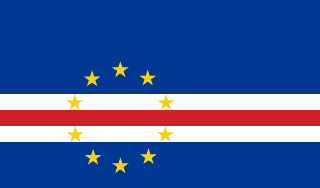
\includegraphics[width=0.3\textwidth]{flags/cv.png}}{
\begin{tabular}{m{3cm} m{5cm}} \textbf{Cape Verde} & \textbf{佛得角} \\[0.5em] \multicolumn{1}{m{3cm}}{\raggedright Praia\\普拉亚\\Portuguese / Creole\\葡萄牙语 / 克里奥尔语} &
\raggedright \textbf{Fact:} En Cabo Verde se celebra el carnaval al ritmo de música criolla, pero con trajes que parecen sacados de Río de Janeiro?
\end{tabular}
}
\card{\centering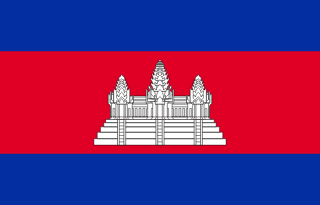
\includegraphics[width=0.3\textwidth]{flags/kh.png}}{
\begin{tabular}{m{3cm} m{5cm}} \textbf{Cambodia} & \textbf{柬埔寨} \\[0.5em] \multicolumn{1}{m{3cm}}{\raggedright Phnom Penh\\金边\\Khmer\\高棉语} &
\raggedright \textbf{Fact:} El templo de Angkor Wat es tan grande que aparece en la bandera de Camboya. ¡Es el único país con un edificio real en su bandera!
\end{tabular}
}
\card{\centering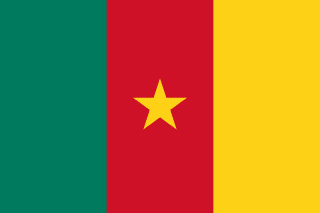
\includegraphics[width=0.3\textwidth]{flags/cm.png}}{
\begin{tabular}{m{3cm} m{5cm}} \textbf{Cameroon} & \textbf{喀麦隆} \\[0.5em] \multicolumn{1}{m{3cm}}{\raggedright Yaoundé\\雅温得\\French / English\\法语 / 英语} &
\raggedright \textbf{Fact:} Camerún es llamado “África en miniatura” porque tiene todos los climas y paisajes del continente. ¡Un resumen geográfico!
\end{tabular}
}
\card{\centering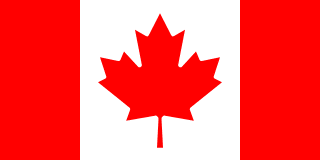
\includegraphics[width=0.3\textwidth]{flags/ca.png}}{
\begin{tabular}{m{3cm} m{5cm}} \textbf{Canada} & \textbf{加拿大} \\[0.5em] \multicolumn{1}{m{3cm}}{\raggedright Ottawa\\渥太华\\English / French\\英语 / 法语} &
\raggedright \textbf{Fact:} En Canadá puedes enviarle una carta a Santa Claus y él te responde? Solo escribe Santa Claus, North Pole, H0H 0H0, Canada… ¡y los elfos voluntarios del correo la responden en más de 30 idiomas!
\end{tabular}
}
\card{\centering
\includegraphics[width=0.3\textwidth]{flags/qa.png}}{
\begin{tabular}{m{3cm} m{5cm}} \textbf{Qatar} & \textbf{卡塔尔} \\[0.5em] \multicolumn{1}{m{3cm}}{\raggedright Doha\\多哈\\Arabic\\阿拉伯语} &
\raggedright \textbf{Fact:} Catar tiene estadios con aire acondicionado al aire libre para combatir el calor del desierto. ¡Fútbol fresco en pleno sol!
\end{tabular}
}
\card{\centering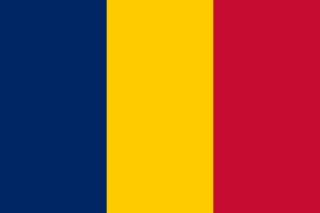
\includegraphics[width=0.3\textwidth]{flags/td.png}}{
\begin{tabular}{m{3cm} m{5cm}} \textbf{Chad} & \textbf{乍得} \\[0.5em] \multicolumn{1}{m{3cm}}{\raggedright N'Djamena\\恩贾梅纳\\French / Arabic\\法语 / 阿拉伯语} &
\raggedright \textbf{Fact:} El lago Chad ha cambiado de tamaño tan dramáticamente que parece un truco de magia cartográfica. ¡Se ha encogido más del 90\%!
\end{tabular}
}
\card{\centering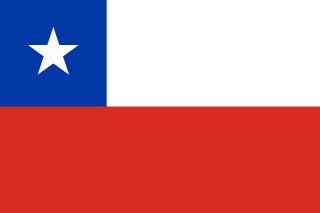
\includegraphics[width=0.3\textwidth]{flags/cl.png}}{
\begin{tabular}{m{3cm} m{5cm}} \textbf{Chile} & \textbf{智利} \\[0.5em] \multicolumn{1}{m{3cm}}{\raggedright Santiago\\圣地亚哥\\Spanish\\西班牙语} &
\raggedright \textbf{Fact:} Chile es tan largo que atraviesa casi todos los climas del planeta. ¡Desde desiertos hasta glaciares!
\end{tabular}
}
\card{\centering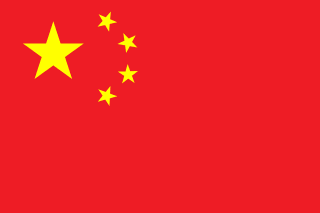
\includegraphics[width=0.3\textwidth]{flags/cn.png}}{
\begin{tabular}{m{3cm} m{5cm}} \textbf{China} & \textbf{中国} \\[0.5em] \multicolumn{1}{m{3cm}}{\raggedright Beijing\\北京\\Chinese\\中文 (普通话)} &
\raggedright \textbf{Fact:} En China existe un puente de cristal colgante que cruje cuando lo pisas… ¡a propósito! Para añadir emoción.
\end{tabular}
}
\card{\centering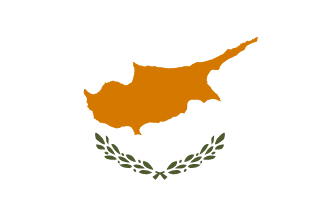
\includegraphics[width=0.3\textwidth]{flags/cy.png}}{
\begin{tabular}{m{3cm} m{5cm}} \textbf{Cyprus} & \textbf{塞浦路斯} \\[0.5em] \multicolumn{1}{m{3cm}}{\raggedright Nicosia\\尼科西亚\\Greek / Turkish\\希腊语 / 土耳其语} &
\raggedright \textbf{Fact:} En Chipre hay una ciudad que es zona de nadie desde 1974, completamente congelada en el tiempo. Se llama Varosha.
\end{tabular}
}
\card{\centering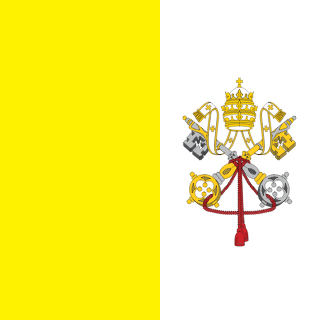
\includegraphics[width=0.3\textwidth]{flags/va.png}}{
\begin{tabular}{m{3cm} m{5cm}} \textbf{Vatican City} & \textbf{梵蒂冈} \\[0.5em] \multicolumn{1}{m{3cm}}{\raggedright Vatican City\\梵蒂冈\\Latin / Italian\\拉丁语 / 意大利语} &
\raggedright \textbf{Fact:} El Vaticano tiene su propia farmacia, su propio servicio postal y hasta su propio equipo de críquet. ¡Un país mini con servicios maxi!
\end{tabular}
}
\card{\centering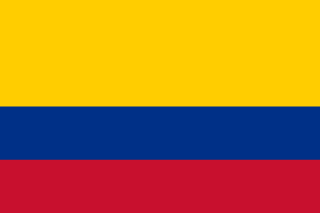
\includegraphics[width=0.3\textwidth]{flags/co.png}}{
\begin{tabular}{m{3cm} m{5cm}} \textbf{Colombia} & \textbf{哥伦比亚} \\[0.5em] \multicolumn{1}{m{3cm}}{\raggedright Bogota\\波哥大\\Spanish\\西班牙语} &
\raggedright \textbf{Fact:} En Colombia hay un río que cambia de color como un arcoíris líquido. Se llama Caño Cristales.
\end{tabular}
}
\card{\centering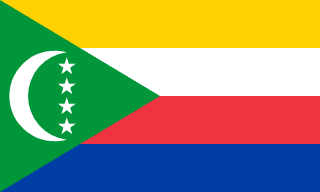
\includegraphics[width=0.3\textwidth]{flags/km.png}}{
\begin{tabular}{m{3cm} m{5cm}} \textbf{Comoros} & \textbf{科摩罗} \\[0.5em] \multicolumn{1}{m{3cm}}{\raggedright Moroni\\莫罗尼\\Arabic / French / Comorian\\阿拉伯语 / 法语 / 科摩罗语} &
\raggedright \textbf{Fact:} Las Comoras son uno de los pocos países donde el perfume es un pilar económico. ¡Exportan toneladas de ylang-ylang!
\end{tabular}
}
\card{\centering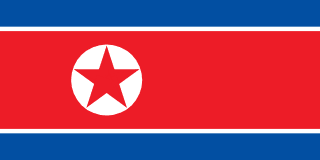
\includegraphics[width=0.3\textwidth]{flags/kp.png}}{
\begin{tabular}{m{3cm} m{5cm}} \textbf{North Corea} & \textbf{朝鲜} \\[0.5em] \multicolumn{1}{m{3cm}}{\raggedright Pyongyang\\平壤\\Corean\\朝鲜语} &
\raggedright \textbf{Fact:} En Corea del Norte el calendario empieza en 1912, año del nacimiento de Kim Il-sung. ¡Están en otro siglo!
\end{tabular}
}
\card{\centering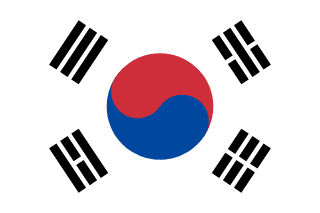
\includegraphics[width=0.3\textwidth]{flags/kr.png}}{
\begin{tabular}{m{3cm} m{5cm}} \textbf{South Corea} & \textbf{韩国} \\[0.5em] \multicolumn{1}{m{3cm}}{\raggedright Seoul\\首尔\\Corean\\韩语} &
\raggedright \textbf{Fact:} En Corea del Sur los bebés nacen con un año de edad? ¡Tienes un año antes de soplar tu primera vela!
\end{tabular}
}
\card{\centering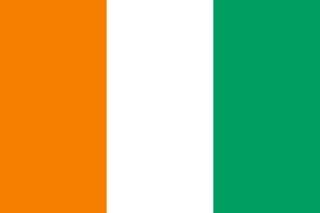
\includegraphics[width=0.3\textwidth]{flags/ci.png}}{
\begin{tabular}{m{3cm} m{5cm}} \textbf{Ivory Coast} & \textbf{科特迪瓦} \\[0.5em] \multicolumn{1}{m{3cm}}{\raggedright Yamoussoukro\\亚穆苏克罗\\French\\法语} &
\raggedright \textbf{Fact:} Costa de Marfil es el mayor productor de cacao del mundo, pero muchos agricultores nunca han probado chocolate.
\end{tabular}
}
\card{\centering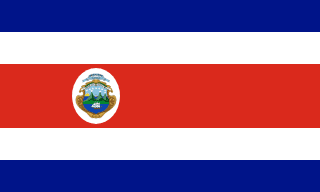
\includegraphics[width=0.3\textwidth]{flags/cr.png}}{
\begin{tabular}{m{3cm} m{5cm}} \textbf{Costa Rica} & \textbf{哥斯达黎加} \\[0.5em] \multicolumn{1}{m{3cm}}{\raggedright San José\\圣何塞\\Spanish\\西班牙语} &
\raggedright \textbf{Fact:} Costa Rica no tiene ejército desde 1949. Prefirió gastar en educación y salud.
\end{tabular}
}
\card{\centering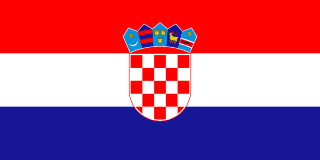
\includegraphics[width=0.3\textwidth]{flags/hr.png}}{
\begin{tabular}{m{3cm} m{5cm}} \textbf{Croatia} & \textbf{克罗地亚} \\[0.5em] \multicolumn{1}{m{3cm}}{\raggedright Zagreb\\萨格勒布\\Croatian\\克罗地亚语} &
\raggedright \textbf{Fact:} La corbata moderna se originó en Croacia. De ahí viene la palabra “cravat”.
\end{tabular}
}
\card{\centering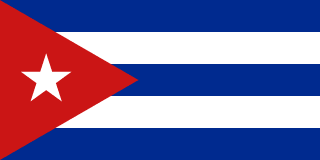
\includegraphics[width=0.3\textwidth]{flags/cu.png}}{
\begin{tabular}{m{3cm} m{5cm}} \textbf{Cuba} & \textbf{古巴} \\[0.5em] \multicolumn{1}{m{3cm}}{\raggedright Havana\\哈瓦那\\Spanish\\西班牙语} &
\raggedright \textbf{Fact:} En Cuba los coches clásicos de los años 50 siguen rodando gracias a una increíble creatividad mecánica.
\end{tabular}
}
\card{\centering\includegraphics[width=0.3\textwidth]{flags/cw.png}}{
\begin{tabular}{m{3cm} m{5cm}} \textbf{Curaçao} & \textbf{库拉索} \\[0.5em] \multicolumn{1}{m{3cm}}{\raggedright Willemstad\\威廉斯塔德\\Papiamento / Dutch / English\\帕皮阿门托语 / 荷兰语, 英语} &
\raggedright \textbf{Fact:} El licor azul Curazao no es naturalmente azul. Se le añade colorante, pero su sabor cítrico es 100\% real.
\end{tabular}
}
\card{\centering\includegraphics[width=0.3\textwidth]{flags/dk.png}}{
\begin{tabular}{m{3cm} m{5cm}} \textbf{Denmark} & \textbf{丹麦} \\[0.5em] \multicolumn{1}{m{3cm}}{\raggedright Copenhagen\\哥本哈根\\Danish\\丹麦语} &
\raggedright \textbf{Fact:} Dinamarca es uno de los países más felices del mundo… y que tiene un museo dedicado a la felicidad?
\end{tabular}
}
\card{\centering\includegraphics[width=0.3\textwidth]{flags/dm.png}}{
\begin{tabular}{m{3cm} m{5cm}} \textbf{Dominica} & \textbf{多米尼加} \\[0.5em] \multicolumn{1}{m{3cm}}{\raggedright Roseau\\罗索\\English / Creole\\英语 / 克里奥尔语} &
\raggedright \textbf{Fact:} Dominica tiene el segundo lago hirviente más grande del mundo. ¡Una sopa geotérmica gigante!
\end{tabular}
}
\card{\centering\includegraphics[width=0.3\textwidth]{flags/ec.png}}{
\begin{tabular}{m{3cm} m{5cm}} \textbf{Ecuador} & \textbf{厄瓜多尔} \\[0.5em] \multicolumn{1}{m{3cm}}{\raggedright Quito\\基多\\Spanish\\西班牙语} &
\raggedright \textbf{Fact:} En Ecuador puedes pararte con un pie en el hemisferio norte y otro en el sur al mismo tiempo.
\end{tabular}
}
\card{\centering\includegraphics[width=0.3\textwidth]{flags/eg.png}}{
\begin{tabular}{m{3cm} m{5cm}} \textbf{Egypt} & \textbf{埃及} \\[0.5em] \multicolumn{1}{m{3cm}}{\raggedright Cairo\\开罗\\Arabic\\阿拉伯语} &
\raggedright \textbf{Fact:} Cleopatra vivió más cerca del iPhone que de la construcción de las pirámides.
\end{tabular}
}
\card{\centering\includegraphics[width=0.3\textwidth]{flags/sv.png}}{
\begin{tabular}{m{3cm} m{5cm}} \textbf{El Salvador} & \textbf{萨尔瓦多} \\[0.5em] \multicolumn{1}{m{3cm}}{\raggedright San Salvador\\圣萨尔瓦多\\Spanish\\西班牙语} &
\raggedright \textbf{Fact:} El Salvador es el único país centroamericano sin costa en el mar Caribe, pero tiene fabulosas olas del Pacífico.
\end{tabular}
}
\card{\centering\includegraphics[width=0.3\textwidth]{flags/ae.png}}{
\begin{tabular}{m{3cm} m{5cm}} \textbf{United Arab Emirates} & \textbf{阿联酋} \\[0.5em] \multicolumn{1}{m{3cm}}{\raggedright Abu Dhabi\\阿布扎比\\Arabic\\阿拉伯语} &
\raggedright \textbf{Fact:} Dubái tiene un cajero automático que dispensa lingotes de oro en lugar de efectivo.
\end{tabular}
}
\card{\centering\includegraphics[width=0.3\textwidth]{flags/er.png}}{
\begin{tabular}{m{3cm} m{5cm}} \textbf{Eritrea} & \textbf{厄立特里亚} \\[0.5em] \multicolumn{1}{m{3cm}}{\raggedright Asmara\\阿斯马拉\\Tigrinya / Arabic\\提格利尼亚语 / 阿拉伯语} &
\raggedright \textbf{Fact:} Eritrea tiene más bicicletas por habitante que coches. ¡Dos ruedas mandan.
\end{tabular}
}
\card{\centering\includegraphics[width=0.3\textwidth]{flags/blank.png}}{
\begin{tabular}{m{3cm} m{5cm}} \textbf{Scotland} & \textbf{苏格兰} \\[0.5em] \multicolumn{1}{m{3cm}}{\raggedright Edinburgh\\爱丁堡\\English / Scottish Gaelic\\英语 / 苏格兰盖尔语} &
\raggedright \textbf{Fact:} En Escocia hay más gaitas que Starbucks. Y probablemente más ovejas también.
\end{tabular}
}
\card{\centering\includegraphics[width=0.3\textwidth]{flags/sk.png}}{
\begin{tabular}{m{3cm} m{5cm}} \textbf{Slovakia} & \textbf{斯洛伐克} \\[0.5em] \multicolumn{1}{m{3cm}}{\raggedright Bratislava\\布拉迪斯拉发\\Slovak\\斯洛伐克语} &
\raggedright \textbf{Fact:} Eslovaquia tiene más de 6,000 cuevas. ¡Hasta Batman se perdería!
\end{tabular}
}
\card{\centering\includegraphics[width=0.3\textwidth]{flags/si.png}}{
\begin{tabular}{m{3cm} m{5cm}} \textbf{Slovenia} & \textbf{斯洛文尼亚} \\[0.5em] \multicolumn{1}{m{3cm}}{\raggedright Ljubljana\\卢布尔雅那\\Slovenian\\斯洛文尼亚语} &
\raggedright \textbf{Fact:} Eslovenia es el hogar del lago Bled, famoso por su isla pintoresca y su castillo medieval.
\end{tabular}
}
\card{\centering\includegraphics[width=0.3\textwidth]{flags/es.png}}{
\begin{tabular}{m{3cm} m{5cm}} \textbf{Spain} & \textbf{西班牙} \\[0.5em] \multicolumn{1}{m{3cm}}{\raggedright Madrid\\马德里\\Spanish\\西班牙语} &
\raggedright \textbf{Fact:} En España hay más bares que en cualquier otro país del mundo ¡Cada esquina tiene un lugar para una tapa!
\end{tabular}
}
\card{\centering\includegraphics[width=0.3\textwidth]{flags/us.png}}{
\begin{tabular}{m{3cm} m{5cm}} \textbf{United States} & \textbf{美国} \\[0.5em] \multicolumn{1}{m{3cm}}{\raggedright Washington D.C\\华盛顿特区\\English\\英语} &
\raggedright \textbf{Fact:} Estados Unidos tiene más de 300,000,000 de coches. ¡Eso es más que la población de muchos países!
\end{tabular}
}
\card{\centering\includegraphics[width=0.3\textwidth]{flags/ee.png}}{
\begin{tabular}{m{3cm} m{5cm}} \textbf{Estonia} & \textbf{爱沙尼亚} \\[0.5em] \multicolumn{1}{m{3cm}}{\raggedright Tallinn\\塔林\\Estonian\\爱沙尼亚语} &
\raggedright \textbf{Fact:} Estonia tiene la mayor cantidad de e-residentes del mundo. ¡Puedes ser residente de Estonia sin pisar el país!
\end{tabular}
}
\card{\centering\includegraphics[width=0.3\textwidth]{flags/et.png}}{
\begin{tabular}{m{3cm} m{5cm}} \textbf{Ethiopia} & \textbf{埃塞俄比亚} \\[0.5em] \multicolumn{1}{m{3cm}}{\raggedright Addis Ababa\\亚的斯亚贝巴\\Amharic\\阿姆哈拉语} &
\raggedright \textbf{Fact:} En Etiopía se usa un calendario diferente al del resto del mundo. ¡Están 7-8 años atrás!
\end{tabular}
}
\card{\centering\includegraphics[width=0.3\textwidth]{flags/ph.png}}{
\begin{tabular}{m{3cm} m{5cm}} \textbf{Philippines} & \textbf{菲律宾} \\[0.5em] \multicolumn{1}{m{3cm}}{\raggedright Manila\\马尼拉\\Tagalog  / English\\塔加洛语 / 英语} &
\raggedright \textbf{Fact:} Filipinas tiene más de 7,000 islas. ¡Es un verdadero paraíso de isla en isla!
\end{tabular}
}
\card{\centering\includegraphics[width=0.3\textwidth]{flags/fi.png}}{
\begin{tabular}{m{3cm} m{5cm}} \textbf{Finland} & \textbf{芬兰} \\[0.5em] \multicolumn{1}{m{3cm}}{\raggedright Helsinki\\赫尔辛基\\Finnish\\芬兰语} &
\raggedright \textbf{Fact:} Finlandia es el hogar de la sauna. ¡Casi todo el mundo tiene una!
\end{tabular}
}
\card{\centering\includegraphics[width=0.3\textwidth]{flags/fj.png}}{
\begin{tabular}{m{3cm} m{5cm}} \textbf{Fiji} & \textbf{斐济} \\[0.5em] \multicolumn{1}{m{3cm}}{\raggedright Suva\\苏瓦\\Fijian / English / Hindi\\斐济语 / 英语 / 印地语} &
\raggedright \textbf{Fact:} Fiyi tiene más de 300 islas, pero solo unas pocas están habitadas.
\end{tabular}
}
\card{\centering\includegraphics[width=0.3\textwidth]{flags/fr.png}}{
\begin{tabular}{m{3cm} m{5cm}} \textbf{France} & \textbf{法国} \\[0.5em] \multicolumn{1}{m{3cm}}{\raggedright Paris\\巴黎\\French\\法语} &
\raggedright \textbf{Fact:} La Torre Eiffel podría crecer hasta 15 cm en verano debido al calor.
\end{tabular}
}
\card{\centering\includegraphics[width=0.3\textwidth]{flags/ga.png}}{
\begin{tabular}{m{3cm} m{5cm}} \textbf{Gabon} & \textbf{加蓬} \\[0.5em] \multicolumn{1}{m{3cm}}{\raggedright Libreville\\利伯维尔\\French\\法语} &
\raggedright \textbf{Fact:}  Gabón tiene uno de los últimos bosques lluviosos intactos del mundo.
\end{tabular}
}
\card{\centering\includegraphics[width=0.3\textwidth]{flags/xw.png}}{
\begin{tabular}{m{3cm} m{5cm}} \textbf{Wales} & \textbf{威尔士} \\[0.5em] \multicolumn{1}{m{3cm}}{\raggedright Cardiff\\卡迪夫\\Welsh / English\\威尔士语 / 英语} &
\raggedright \textbf{Fact:} Gales tiene un pueblo con el nombre más largo de Europa. Se llama “Llanfair­pwllgwyngyllgogerychwyrndrobwllllantysiliogogogoch”.
\end{tabular}
}
\card{\centering\includegraphics[width=0.3\textwidth]{flags/gm.png}}{
\begin{tabular}{m{3cm} m{5cm}} \textbf{Gambia} & \textbf{冈比亚} \\[0.5em] \multicolumn{1}{m{3cm}}{\raggedright Banjul\\班珠尔\\English\\英语} &
\raggedright \textbf{Fact:} Gambia es el país más pequeño de África, pero tiene una increíble diversidad de fauna.
\end{tabular}
}
\card{\centering\includegraphics[width=0.3\textwidth]{flags/ge.png}}{
\begin{tabular}{m{3cm} m{5cm}} \textbf{Georgia} & \textbf{格鲁吉亚} \\[0.5em] \multicolumn{1}{m{3cm}}{\raggedright Tbilisi\\第比利斯\\Georgian\\格鲁吉亚语} &
\raggedright \textbf{Fact:} Georgia es famosa por ser el lugar de nacimiento del vino, con más de 8,000 años de tradición vinícola.
\end{tabular}
}
\card{\centering\includegraphics[width=0.3\textwidth]{flags/gh.png}}{
\begin{tabular}{m{3cm} m{5cm}} \textbf{Ghana} & \textbf{加纳} \\[0.5em] \multicolumn{1}{m{3cm}}{\raggedright Accra\\阿克拉\\English\\英语} &
\raggedright \textbf{Fact:} Ghana fue el primer país africano en obtener la independencia del Reino Unido.
\end{tabular}
}
\card{\centering\includegraphics[width=0.3\textwidth]{flags/gi.png}}{
\begin{tabular}{m{3cm} m{5cm}} \textbf{Gibraltar} & \textbf{直布罗陀} \\[0.5em] \multicolumn{1}{m{3cm}}{\raggedright Gibraltar\\直布罗陀\\English\\英语} &
\raggedright \textbf{Fact:} Gibraltar es el hogar de los monos salvajes, conocidos como los “macacos de Gibraltar”.
\end{tabular}
}
\card{\centering\includegraphics[width=0.3\textwidth]{flags/gd.png}}{
\begin{tabular}{m{3cm} m{5cm}} \textbf{Grenada} & \textbf{格林纳达} \\[0.5em] \multicolumn{1}{m{3cm}}{\raggedright St. George's\\圣乔治\\English\\英语} &
\raggedright \textbf{Fact:} Granada es famosa por sus plantaciones de nuez moscada y especias.
\end{tabular}
}
\card{\centering\includegraphics[width=0.3\textwidth]{flags/gr.png}}{
\begin{tabular}{m{3cm} m{5cm}} \textbf{Greece} & \textbf{希腊} \\[0.5em] \multicolumn{1}{m{3cm}}{\raggedright Athens\\雅典\\Greek\\希腊语} &
\raggedright \textbf{Fact:} Grecia tiene más de 200 islas habitadas. ¡Es un verdadero paraíso de agua azul y arquitectura antigua!
\end{tabular}
}
\card{\centering\includegraphics[width=0.3\textwidth]{flags/gl.png}}{
\begin{tabular}{m{3cm} m{5cm}} \textbf{Greenland} & \textbf{格林兰} \\[0.5em] \multicolumn{1}{m{3cm}}{\raggedright Nuuk\\努克\\Greenlandic / Danish\\格陵兰语 / 丹麦语} &
\raggedright \textbf{Fact:} El 80\% de Groenlandia está cubierto por hielo.
\end{tabular}
}
\card{\centering\includegraphics[width=0.3\textwidth]{flags/gt.png}}{
\begin{tabular}{m{3cm} m{5cm}} \textbf{Guatemala} & \textbf{危地马拉} \\[0.5em] \multicolumn{1}{m{3cm}}{\raggedright Guatemala City\\危地马拉市\\Spanish\\西班牙语} &
\raggedright \textbf{Fact:} Guatemala fue el hogar de la antigua civilización maya, y tiene una de las pirámides más grandes de la región.
\end{tabular}
}
\card{\centering\includegraphics[width=0.3\textwidth]{flags/gy.png}}{
\begin{tabular}{m{3cm} m{5cm}} \textbf{Guyana} & \textbf{圭亚那} \\[0.5em] \multicolumn{1}{m{3cm}}{\raggedright Georgetown\\乔治敦\\English\\英语} &
\raggedright \textbf{Fact:} Guyana es el único país sudamericano donde el inglés es el idioma oficial, pero su acento es tan único que incluso los británicos necesitan subtítulos. ¡Hablan inglés, pero al estilo “solo Guyana lo entiende”!
\end{tabular}
}
\card{\centering\includegraphics[width=0.3\textwidth]{flags/gn.png}}{
\begin{tabular}{m{3cm} m{5cm}} \textbf{Guinea} & \textbf{几内亚} \\[0.5em] \multicolumn{1}{m{3cm}}{\raggedright Conakry\\科纳克里\\French\\法语} &
\raggedright \textbf{Fact:} Guinea fue uno de los países más ricos en bauxita, un mineral clave para la fabricación de aluminio.
\end{tabular}
}
\card{\centering\includegraphics[width=0.3\textwidth]{flags/gw.png}}{
\begin{tabular}{m{3cm} m{5cm}} \textbf{Guinea-Bissau} & \textbf{几内亚比绍} \\[0.5em] \multicolumn{1}{m{3cm}}{\raggedright Bissau\\比绍\\Portuguese\\葡萄牙语} &
\raggedright \textbf{Fact:} Guinea-Bisáu es conocida por su salsa de palma, un ingrediente fundamental en su gastronomía local.
\end{tabular}
}
\card{\centering\includegraphics[width=0.3\textwidth]{flags/gq.png}}{
\begin{tabular}{m{3cm} m{5cm}} \textbf{Equatorial Guinea} & \textbf{赤道几内亚} \\[0.5em] \multicolumn{1}{m{3cm}}{\raggedright Malabo\\马拉博\\Spanish\\西班牙语} &
\raggedright \textbf{Fact:} Guinea Ecuatorial tiene dos capitales, Malabo (en la isla de Bioko) y Oyala (en el continente).
\end{tabular}
}
\card{\centering\includegraphics[width=0.3\textwidth]{flags/ht.png}}{
\begin{tabular}{m{3cm} m{5cm}} \textbf{Haiti} & \textbf{海地} \\[0.5em] \multicolumn{1}{m{3cm}}{\raggedright Port-au-Prince\\太子港\\Haitian Creole, French\\海地克里奥尔语 / 法语} &
\raggedright \textbf{Fact:} Haití es el primer país en América Latina que obtuvo su independencia, tras una exitosa revolución de esclavos.
\end{tabular}
}
\card{\centering\includegraphics[width=0.3\textwidth]{flags/hn.png}}{
\begin{tabular}{m{3cm} m{5cm}} \textbf{Honduras} & \textbf{洪都拉斯} \\[0.5em] \multicolumn{1}{m{3cm}}{\raggedright Tegucigalpa\\特古西加尔巴\\Spanish\\西班牙语} &
\raggedright \textbf{Fact:} Honduras tiene las ruinas mayas de Copán, una de las siete maravillas de la cultura maya.
\end{tabular}
}
\card{\centering\includegraphics[width=0.3\textwidth]{flags/hk.png}}{
\begin{tabular}{m{3cm} m{5cm}} \textbf{Hong Kong} & \textbf{香港} \\[0.5em] \multicolumn{1}{m{3cm}}{\raggedright Hong Kong\\香港\\Cantonese\\粤语} &
\raggedright \textbf{Fact:} Hong Kong tiene una de las ciudades más densamente pobladas del mundo, con rascacielos apilados sobre montañas.
\end{tabular}
}
\card{\centering\includegraphics[width=0.3\textwidth]{flags/hu.png}}{
\begin{tabular}{m{3cm} m{5cm}} \textbf{Hungary} & \textbf{匈牙利} \\[0.5em] \multicolumn{1}{m{3cm}}{\raggedright Budapest\\布达佩斯\\Hungarian\\匈牙利语} &
\raggedright \textbf{Fact:} Hungría es famosa por su lengua única, que no se parece a ninguna otra en Europa.
\end{tabular}
}
\card{\centering\includegraphics[width=0.3\textwidth]{flags/in.png}}{
\begin{tabular}{m{3cm} m{5cm}} \textbf{India} & \textbf{印度} \\[0.5em] \multicolumn{1}{m{3cm}}{\raggedright New Delhi\\新德里\\Hindi / English\\印地语 / 英语} &
\raggedright \textbf{Fact:} India tiene más de 2,000 grupos étnicos diferentes y más de 1,600 idiomas y dialectos.
\end{tabular}
}
\card{\centering\includegraphics[width=0.3\textwidth]{flags/id.png}}{
\begin{tabular}{m{3cm} m{5cm}} \textbf{Indonesia} & \textbf{印度尼西亚} \\[0.5em] \multicolumn{1}{m{3cm}}{\raggedright Jakarta\\雅加达\\Indonesian\\印度尼西亚语} &
\raggedright \textbf{Fact:} Indonesia tiene la mayor cantidad de volcanes activos del mundo.
\end{tabular}
}
\card{\centering\includegraphics[width=0.3\textwidth]{flags/iq.png}}{
\begin{tabular}{m{3cm} m{5cm}} \textbf{Iraq} & \textbf{伊拉克} \\[0.5em] \multicolumn{1}{m{3cm}}{\raggedright Baghdad\\巴格达\\Arabic\\阿拉伯语} &
\raggedright \textbf{Fact:} Irak es el lugar donde se originaron muchas de las primeras civilizaciones, como los sumerios, hace miles de años.
\end{tabular}
}
\card{\centering\includegraphics[width=0.3\textwidth]{flags/ir.png}}{
\begin{tabular}{m{3cm} m{5cm}} \textbf{Iran} & \textbf{伊朗} \\[0.5em] \multicolumn{1}{m{3cm}}{\raggedright Tehran\\德黑兰\\Persian\\波斯语} &
\raggedright \textbf{Fact:} Irán es famoso por sus hermosos jardines persas, que están diseñados para reflejar el paraíso.
\end{tabular}
}
\card{\centering\includegraphics[width=0.3\textwidth]{flags/ie.png}}{
\begin{tabular}{m{3cm} m{5cm}} \textbf{Ireland} & \textbf{爱尔兰} \\[0.5em] \multicolumn{1}{m{3cm}}{\raggedright Dublin\\都柏林\\Irish / English\\爱尔兰语 / 英语} &
\raggedright \textbf{Fact:} Irlanda es conocida por sus paisajes verdes y pintorescos, que la han hecho famosa como la Isla Esmeralda.
\end{tabular}
}
\card{\centering\includegraphics[width=0.3\textwidth]{flags/xn.png}}{
\begin{tabular}{m{3cm} m{5cm}} \textbf{Northern Ireland} & \textbf{北爱尔兰} \\[0.5em] \multicolumn{1}{m{3cm}}{\raggedright Belfast \\贝尔法斯特\\English\\英语} &
\raggedright \textbf{Fact:} Irlanda del Norte puedes visitar la famosa Calzada del Gigante, una formación geológica única de columnas de basalto.
\end{tabular}
}
\card{\centering\includegraphics[width=0.3\textwidth]{flags/is.png}}{
\begin{tabular}{m{3cm} m{5cm}} \textbf{Iceland} & \textbf{冰岛} \\[0.5em] \multicolumn{1}{m{3cm}}{\raggedright Reykjavik\\雷克雅未克\\Icelandic\\冰岛语} &
\raggedright \textbf{Fact:} Islandia es uno de los países con más géiseres y aguas termales del mundo.
\end{tabular}
}
\card{\centering\includegraphics[width=0.3\textwidth]{flags/ck.png}}{
\begin{tabular}{m{3cm} m{5cm}} \textbf{Cook Islands} & \textbf{库克群岛} \\[0.5em] \multicolumn{1}{m{3cm}}{\raggedright Avarua\\阿瓦鲁阿\\Cook Islands Māori / English\\库克岛毛利语 / 英语} &
\raggedright \textbf{Fact:} Las Islas Cook tienen uno de los cielos más estrellados del planeta, ideal para la observación astronómica.
\end{tabular}
}
\card{\centering\includegraphics[width=0.3\textwidth]{flags/fo.png}}{
\begin{tabular}{m{3cm} m{5cm}} \textbf{Faroe Islands} & \textbf{法罗群岛} \\[0.5em] \multicolumn{1}{m{3cm}}{\raggedright Tórshavn\\托尔斯港\\Faroese / Danish\\法罗语 / 丹麦语} &
\raggedright \textbf{Fact:} Las Islas Feroe son famosas por su pesca y sus coloridos pueblos ubicados en montañas escarpadas.
\end{tabular}
}
\card{\centering\includegraphics[width=0.3\textwidth]{flags/mh.png}}{
\begin{tabular}{m{3cm} m{5cm}} \textbf{Marshall Islands} & \textbf{马绍尔群岛} \\[0.5em] \multicolumn{1}{m{3cm}}{\raggedright Majuro\\马朱罗\\Marshallese / English\\马绍尔语 / 英语} &
\raggedright \textbf{Fact:} Las Islas Marshall fueron el sitio de numerosas pruebas nucleares durante la Guerra Fría.
\end{tabular}
}
\card{\centering\includegraphics[width=0.3\textwidth]{flags/sb.png}}{
\begin{tabular}{m{3cm} m{5cm}} \textbf{Solomon Islands} & \textbf{所罗门群岛} \\[0.5em] \multicolumn{1}{m{3cm}}{\raggedright Honiara\\所罗门群岛\\English\\英语} &
\raggedright \textbf{Fact:} Las Islas Salomón tienen algunas de las mejores aguas cristalinas del mundo, ideales para el buceo.
\end{tabular}
}
\card{\centering\includegraphics[width=0.3\textwidth]{flags/il.png}}{
\begin{tabular}{m{3cm} m{5cm}} \textbf{Israel} & \textbf{以色列} \\[0.5em] \multicolumn{1}{m{3cm}}{\raggedright Jerusalem\\耶路撒冷\\Hebrew\\希伯来语} &
\raggedright \textbf{Fact:} Israel se encuentran tanto el Mar Muerto, el punto más bajo de la Tierra, como los restos de la antigua ciudad de Jerusalén.
\end{tabular}
}
\card{\centering\includegraphics[width=0.3\textwidth]{flags/it.png}}{
\begin{tabular}{m{3cm} m{5cm}} \textbf{Italy} & \textbf{意大利} \\[0.5em] \multicolumn{1}{m{3cm}}{\raggedright Rome\\罗马\\Italian\\意大利语} &
\raggedright \textbf{Fact:} Italia es el hogar de la pizza, que originalmente se inventó en Nápoles en el siglo XVIII.
\end{tabular}
}
\card{\centering\includegraphics[width=0.3\textwidth]{flags/jm.png}}{
\begin{tabular}{m{3cm} m{5cm}} \textbf{Jamaica} & \textbf{牙买加} \\[0.5em] \multicolumn{1}{m{3cm}}{\raggedright Kingston\\金斯敦\\English\\英语} &
\raggedright \textbf{Fact:} Jamaica es la cuna del reggae, y su famoso cantante Bob Marley sigue siendo una leyenda mundial de la música.
\end{tabular}
}
\card{\centering\includegraphics[width=0.3\textwidth]{flags/jp.png}}{
\begin{tabular}{m{3cm} m{5cm}} \textbf{Japan} & \textbf{日本} \\[0.5em] \multicolumn{1}{m{3cm}}{\raggedright Tokyo\\东京\\Japanese\\日语} &
\raggedright \textbf{Fact:} Japón tiene más de 3,000 islas, y que el monte Fuji es su volcán más famoso.
\end{tabular}
}
\card{\centering\includegraphics[width=0.3\textwidth]{flags/jo.png}}{
\begin{tabular}{m{3cm} m{5cm}} \textbf{Jordan} & \textbf{约旦} \\[0.5em] \multicolumn{1}{m{3cm}}{\raggedright Amman\\安曼\\Arabic\\阿拉伯语} &
\raggedright \textbf{Fact:} En Jordania se encuentra Petra, la antigua ciudad esculpida en piedra roja, famosa por sus monumentos tallados
\end{tabular}
}
\card{\centering\includegraphics[width=0.3\textwidth]{flags/kz.png}}{
\begin{tabular}{m{3cm} m{5cm}} \textbf{Kazakhstan} & \textbf{哈萨克斯坦} \\[0.5em] \multicolumn{1}{m{3cm}}{\raggedright Astana\\阿斯塔納\\Kazakh / Russian\\哈萨克语 / 俄语} &
\raggedright \textbf{Fact:} Kazajistán es el país más grande de Asia Central y tiene vastas estepas, donde las yurtas tradicionales aún son comunes.
\end{tabular}
}
\card{\centering\includegraphics[width=0.3\textwidth]{flags/ke.png}}{
\begin{tabular}{m{3cm} m{5cm}} \textbf{Kenya} & \textbf{肯尼亚} \\[0.5em] \multicolumn{1}{m{3cm}}{\raggedright Nairobi\\内罗毕\\Swahili\\斯瓦希里语} &
\raggedright \textbf{Fact:} Kenia es famosa por su vida salvaje, siendo hogar del famoso Gran Migración de los ñus en el Masai Mara.
\end{tabular}
}
\card{\centering\includegraphics[width=0.3\textwidth]{flags/ki.png}}{
\begin{tabular}{m{3cm} m{5cm}} \textbf{Kiribati} & \textbf{基里巴斯} \\[0.5em] \multicolumn{1}{m{3cm}}{\raggedright Tarawa\\塔拉瓦\\Gilbertese / English\\基尔伯特语 / 英语} &
\raggedright \textbf{Fact:} Kiribati está compuesto por 33 atolones y es uno de los países más vulnerables al cambio climático.
\end{tabular}
}
\card{\centering\includegraphics[width=0.3\textwidth]{flags/xk.png}}{
\begin{tabular}{m{3cm} m{5cm}} \textbf{Kosovo} & \textbf{科索沃} \\[0.5em] \multicolumn{1}{m{3cm}}{\raggedright Pristina\\普里什蒂纳\\Albanian / Serbian\\阿尔巴尼亚语 / 塞尔维亚语} &
\raggedright \textbf{Fact:} Kosovo declaró su independencia de Serbia en 2008, y su bandera tiene estrellas amarillas sobre un fondo azul.
\end{tabular}
}
\card{\centering\includegraphics[width=0.3\textwidth]{flags/kw.png}}{
\begin{tabular}{m{3cm} m{5cm}} \textbf{Kuwait} & \textbf{科威特} \\[0.5em] \multicolumn{1}{m{3cm}}{\raggedright Kuwait City\\科威特城\\Arabic\\阿拉伯语} &
\raggedright \textbf{Fact:} Kuwait tiene uno de los puertos más importantes del Golfo Pérsico y es famoso por su rascacielos Burj Mubarak Al-Kabir.
\end{tabular}
}
\card{\centering\includegraphics[width=0.3\textwidth]{flags/la.png}}{
\begin{tabular}{m{3cm} m{5cm}} \textbf{Laos} & \textbf{老挝} \\[0.5em] \multicolumn{1}{m{3cm}}{\raggedright Vientiane\\万象\\Lao\\老挝语} &
\raggedright \textbf{Fact:} Laos es uno de los países más pobres del sudeste asiático, pero también cuenta con hermosos paisajes montañosos.
\end{tabular}
}
\card{\centering\includegraphics[width=0.3\textwidth]{flags/ls.png}}{
\begin{tabular}{m{3cm} m{5cm}} \textbf{Lesotho} & \textbf{莱索托} \\[0.5em] \multicolumn{1}{m{3cm}}{\raggedright Maseru\\马塞卢\\Sesotho / English\\塞索托语 / 英语} &
\raggedright \textbf{Fact:} Lesoto es uno de los pocos países del mundo que está completamente rodeado por otro país, Sudáfrica.
\end{tabular}
}
\card{\centering\includegraphics[width=0.3\textwidth]{flags/lv.png}}{
\begin{tabular}{m{3cm} m{5cm}} \textbf{Latvia} & \textbf{拉脱维亚} \\[0.5em] \multicolumn{1}{m{3cm}}{\raggedright Riga\\里加\\Latvian\\拉脱维亚语} &
\raggedright \textbf{Fact:} Letonia tiene una de las densidades más altas de bosques en Europa, cubriendo más del 50\% de su territorio.
\end{tabular}
}
\card{\centering\includegraphics[width=0.3\textwidth]{flags/lb.png}}{
\begin{tabular}{m{3cm} m{5cm}} \textbf{Lebanon} & \textbf{黎巴嫩} \\[0.5em] \multicolumn{1}{m{3cm}}{\raggedright Beirut\\贝鲁特\\Arabic\\阿拉伯语} &
\raggedright \textbf{Fact:} Líbano tiene una de las civilizaciones más antiguas del mundo, con sitios arqueológicos como Baalbek que datan de hace 5,000 años.
\end{tabular}
}
\card{\centering\includegraphics[width=0.3\textwidth]{flags/lr.png}}{
\begin{tabular}{m{3cm} m{5cm}} \textbf{Liberia} & \textbf{利比里亚} \\[0.5em] \multicolumn{1}{m{3cm}}{\raggedright Monrovia\\蒙罗维亚\\English\\英语} &
\raggedright \textbf{Fact:} Liberia es el único país en África que fue fundado por antiguos esclavos liberados de Estados Unidos.
\end{tabular}
}
\card{\centering\includegraphics[width=0.3\textwidth]{flags/ly.png}}{
\begin{tabular}{m{3cm} m{5cm}} \textbf{Libya} & \textbf{利比亚} \\[0.5em] \multicolumn{1}{m{3cm}}{\raggedright Tripoli\\的黎波里\\Arabic\\阿拉伯语} &
\raggedright \textbf{Fact:} Libia tiene una de las ciudades más antiguas del mundo, Leptis Magna, que data del siglo VII a.C.
\end{tabular}
}
\card{\centering\includegraphics[width=0.3\textwidth]{flags/li.png}}{
\begin{tabular}{m{3cm} m{5cm}} \textbf{Liechtenstein} & \textbf{列支敦士登} \\[0.5em] \multicolumn{1}{m{3cm}}{\raggedright Vaduz\\瓦杜茨\\German\\德语} &
\raggedright \textbf{Fact:} Liechtenstein es uno de los países más pequeños del mundo, pero también uno de los más ricos per cápita.
\end{tabular}
}
\card{\centering\includegraphics[width=0.3\textwidth]{flags/lt.png}}{
\begin{tabular}{m{3cm} m{5cm}} \textbf{Lithuania} & \textbf{立陶宛} \\[0.5em] \multicolumn{1}{m{3cm}}{\raggedright Vilnius\\维尔纽斯\\Lithuanian\\立陶宛语} &
\raggedright \textbf{Fact:} Lituania es el hogar de la primera universidad en el mundo en enseñar filosofía moderna, la Universidad de Vilna.
\end{tabular}
}
\card{\centering\includegraphics[width=0.3\textwidth]{flags/lu.png}}{
\begin{tabular}{m{3cm} m{5cm}} \textbf{Luxembourg} & \textbf{卢森堡} \\[0.5em] \multicolumn{1}{m{3cm}}{\raggedright Luxembourg\\卢森堡\\Luxembourgish / French / German\\卢森堡语 / 法语 / 德语} &
\raggedright \textbf{Fact:} Luxemburgo es famoso por su pequeño tamaño, pero tiene uno de los estándares de vida más altos del mundo.
\end{tabular}
}
\card{\centering\includegraphics[width=0.3\textwidth]{flags/mo.png}}{
\begin{tabular}{m{3cm} m{5cm}} \textbf{Macao} & \textbf{澳门} \\[0.5em] \multicolumn{1}{m{3cm}}{\raggedright Macao\\澳门\\Chinese / Portuguese\\中文 / 葡萄牙语} &
\raggedright \textbf{Fact:} Macao es conocida como Las Vegas de Asia por sus grandes casinos y su vibrante vida nocturna.
\end{tabular}
}
\card{\centering\includegraphics[width=0.3\textwidth]{flags/mk.png}}{
\begin{tabular}{m{3cm} m{5cm}} \textbf{Noth Macedonia} & \textbf{北马其顿} \\[0.5em] \multicolumn{1}{m{3cm}}{\raggedright Skopje\\斯科普里\\Macedonian\\马其顿语} &
\raggedright \textbf{Fact:} Macedonia del Norte es famosa por su hermoso lago Ohrid, uno de los lagos más antiguos y profundos de Europa.
\end{tabular}
}
\card{\centering\includegraphics[width=0.3\textwidth]{flags/mg.png}}{
\begin{tabular}{m{3cm} m{5cm}} \textbf{Madagascar} & \textbf{马达加斯加} \\[0.5em] \multicolumn{1}{m{3cm}}{\raggedright Antananarivo\\塔那那利佛\\Malagasy / French\\马尔加什语 / 法语} &
\raggedright \textbf{Fact:} Madagascar es hogar de especies únicas como los lémures, que no se encuentran en ningún otro lugar del mundo. ¡Quiero mover el bote!
\end{tabular}
}
\card{\centering\includegraphics[width=0.3\textwidth]{flags/my.png}}{
\begin{tabular}{m{3cm} m{5cm}} \textbf{Malaysia} & \textbf{马来西亚} \\[0.5em] \multicolumn{1}{m{3cm}}{\raggedright Kuala Lumpur\\吉隆坡\\Malay\\马来语} &
\raggedright \textbf{Fact:} Malasia es conocida por su asombroso mix de culturas, combinando tradiciones malayas, chinas e indias.
\end{tabular}
}
\card{\centering\includegraphics[width=0.3\textwidth]{flags/mw.png}}{
\begin{tabular}{m{3cm} m{5cm}} \textbf{Malawi} & \textbf{马拉维} \\[0.5em] \multicolumn{1}{m{3cm}}{\raggedright Lilongwe\\利隆圭\\Chichewa / English\\齐切瓦语 / 英语} &
\raggedright \textbf{Fact:} Malaui es conocida como el Corazón cálido de África debido a la amabilidad de su gente y su clima tropical.
\end{tabular}
}
\card{\centering\includegraphics[width=0.3\textwidth]{flags/mv.png}}{
\begin{tabular}{m{3cm} m{5cm}} \textbf{Maldives} & \textbf{马尔代夫} \\[0.5em] \multicolumn{1}{m{3cm}}{\raggedright Malé\\马累\\Dhivehi\\马尔代夫语} &
\raggedright \textbf{Fact:} Las Maldivas están compuestas por más de 1,000 islas, y muchas de ellas están bajo amenaza por el cambio climático.
\end{tabular}
}
\card{\centering\includegraphics[width=0.3\textwidth]{flags/ml.png}}{
\begin{tabular}{m{3cm} m{5cm}} \textbf{Mali} & \textbf{马里} \\[0.5em] \multicolumn{1}{m{3cm}}{\raggedright Bamako\\巴马科\\French\\法语} &
\raggedright \textbf{Fact:} Malí es famoso por su rica historia, incluyendo el antiguo imperio de Ghana, una de las civilizaciones más poderosas de África.
\end{tabular}
}
\card{\centering\includegraphics[width=0.3\textwidth]{flags/mt.png}}{
\begin{tabular}{m{3cm} m{5cm}} \textbf{Malta} & \textbf{马耳他} \\[0.5em] \multicolumn{1}{m{3cm}}{\raggedright Valletta\\瓦莱塔\\Maltese / English\\马耳他语 / 英语} &
\raggedright \textbf{Fact:} Malta es el hogar de algunas de las estructuras prehistóricas más antiguas de Europa, más antiguas que las pirámides de Egipto.
\end{tabular}
}
\card{\centering\includegraphics[width=0.3\textwidth]{flags/ma.png}}{
\begin{tabular}{m{3cm} m{5cm}} \textbf{Morocco} & \textbf{摩洛哥} \\[0.5em] \multicolumn{1}{m{3cm}}{\raggedright Rabat\\拉巴特\\Arabic\\阿拉伯语} &
\raggedright \textbf{Fact:} Marruecos es conocido por su famosa Plaza Jemaa el-Fna en Marrakech, un centro vibrante de cultura, comida y entretenimiento.
\end{tabular}
}
\card{\centering\includegraphics[width=0.3\textwidth]{flags/mu.png}}{
\begin{tabular}{m{3cm} m{5cm}} \textbf{Mauritius} & \textbf{毛里求斯} \\[0.5em] \multicolumn{1}{m{3cm}}{\raggedright Port-Louis\\路易港\\French\\法语} &
\raggedright \textbf{Fact:} Mauricio fue el hogar del dodo, el ave extinta que se volvió símbolo de extinción.
\end{tabular}
}
\card{\centering\includegraphics[width=0.3\textwidth]{flags/mr.png}}{
\begin{tabular}{m{3cm} m{5cm}} \textbf{Mauritania} & \textbf{毛里塔尼亚} \\[0.5em] \multicolumn{1}{m{3cm}}{\raggedright Nouakchott\\努瓦克肖特\\Arabic / French\\阿拉伯语 / 法语} &
\raggedright \textbf{Fact:} Mauritania es uno de los pocos países en el mundo donde la esclavitud aún persiste en formas modernas.
\end{tabular}
}
\card{\centering\includegraphics[width=0.3\textwidth]{flags/mx.png}}{
\begin{tabular}{m{3cm} m{5cm}} \textbf{Mexico} & \textbf{墨西哥} \\[0.5em] \multicolumn{1}{m{3cm}}{\raggedright Mexico City\\墨西哥城\\Spanish\\西班牙语} &
\raggedright \textbf{Fact:} México es hogar de la antigua ciudad maya de Chichén Itzá, una de las Nuevas Siete Maravillas del Mundo.
\end{tabular}
}
\card{\centering\includegraphics[width=0.3\textwidth]{flags/fm.png}}{
\begin{tabular}{m{3cm} m{5cm}} \textbf{Micronesia} & \textbf{密克罗尼西亚} \\[0.5em] \multicolumn{1}{m{3cm}}{\raggedright Palikir\\帕利基尔\\English\\英语} &
\raggedright \textbf{Fact:} Micronesia está compuesta por más de 600 islas, pero solo unas pocas están habitadas.
\end{tabular}
}
\card{\centering\includegraphics[width=0.3\textwidth]{flags/md.png}}{
\begin{tabular}{m{3cm} m{5cm}} \textbf{Moldova} & \textbf{摩尔多瓦} \\[0.5em] \multicolumn{1}{m{3cm}}{\raggedright Chișinău\\基希讷乌\\Romanain\\罗马尼亚语} &
\raggedright \textbf{Fact:} Moldavia tiene una de las bodegas de vino más grandes del mundo, con más de 200 km de túneles subterráneos.
\end{tabular}
}
\card{\centering\includegraphics[width=0.3\textwidth]{flags/mc.png}}{
\begin{tabular}{m{3cm} m{5cm}} \textbf{Monaco} & \textbf{摩纳哥} \\[0.5em] \multicolumn{1}{m{3cm}}{\raggedright Monaco\\摩纳哥\\French\\法语} &
\raggedright \textbf{Fact:} Mónaco es el segundo país más pequeño del mundo, pero tiene una de las concentraciones más altas de riqueza.
\end{tabular}
}
\card{\centering\includegraphics[width=0.3\textwidth]{flags/mn.png}}{
\begin{tabular}{m{3cm} m{5cm}} \textbf{Mongolia} & \textbf{蒙古} \\[0.5em] \multicolumn{1}{m{3cm}}{\raggedright Ulaanbaatar\\乌兰巴托\\Mongolian\\蒙古语} &
\raggedright \textbf{Fact:} Mongolia es famosa por su cultura nómada, y el Festival Naadam celebra competencias de lucha, carreras de caballos y tiro con arco.
\end{tabular}
}
\card{\centering\includegraphics[width=0.3\textwidth]{flags/ms.png}}{
\begin{tabular}{m{3cm} m{5cm}} \textbf{Montserrat} & \textbf{蒙特塞拉特} \\[0.5em] \multicolumn{1}{m{3cm}}{\raggedright Brades\\布雷兹\\English\\英语} &
\raggedright \textbf{Fact:} Montserrat es una isla volcánica en el Caribe, famosa por su volcán activo, que ha creado una zona de exclusión en gran parte de la isla.
\end{tabular}
}
\card{\centering\includegraphics[width=0.3\textwidth]{flags/me.png}}{
\begin{tabular}{m{3cm} m{5cm}} \textbf{Montenegro} & \textbf{黑山} \\[0.5em] \multicolumn{1}{m{3cm}}{\raggedright Podgorica\\波德戈里察\\Montenegrin\\黑山语} &
\raggedright \textbf{Fact:} Montenegro es famosa por su impresionante costa en el mar Adriático, con hermosas playas y montañas que se encuentran directamente junto al mar.
\end{tabular}
}
\card{\centering\includegraphics[width=0.3\textwidth]{flags/mz.png}}{
\begin{tabular}{m{3cm} m{5cm}} \textbf{Mozambique} & \textbf{莫桑比克} \\[0.5em] \multicolumn{1}{m{3cm}}{\raggedright Maputo\\马普托\\Portuguese\\葡萄牙语} &
\raggedright \textbf{Fact:} Mozambique tiene una de las costas más largas de África, hogar de hermosas islas tropicales y arrecifes de coral.
\end{tabular}
}
\card{\centering\includegraphics[width=0.3\textwidth]{flags/na.png}}{
\begin{tabular}{m{3cm} m{5cm}} \textbf{Namibia} & \textbf{纳米比亚} \\[0.5em] \multicolumn{1}{m{3cm}}{\raggedright Windhoek\\温得和克\\English\\英语} &
\raggedright \textbf{Fact:} Namibia es hogar del desierto de Namib, uno de los desiertos más antiguos del mundo, famoso por sus enormes dunas de arena roja.
\end{tabular}
}
\card{\centering\includegraphics[width=0.3\textwidth]{flags/nr.png}}{
\begin{tabular}{m{3cm} m{5cm}} \textbf{Nauru} & \textbf{瑙鲁} \\[0.5em] \multicolumn{1}{m{3cm}}{\raggedright Yaren\\亚伦\\Nauruan / English\\瑙鲁语 / 英语} &
\raggedright \textbf{Fact:} Nauru es el tercer país más pequeño del mundo por superficie, y su economía fue originalmente basada en la minería de fosfato.
\end{tabular}
}
\card{\centering\includegraphics[width=0.3\textwidth]{flags/np.png}}{
\begin{tabular}{m{3cm} m{5cm}} \textbf{Nepal} & \textbf{尼泊尔} \\[0.5em] \multicolumn{1}{m{3cm}}{\raggedright Katmandhu\\加德满都\\Nepali\\尼泊尔语} &
\raggedright \textbf{Fact:} Nepal es el hogar de la montaña más alta del mundo, el Monte Everest, que atrae a miles de alpinistas cada año.
\end{tabular}
}
\card{\centering\includegraphics[width=0.3\textwidth]{flags/ni.png}}{
\begin{tabular}{m{3cm} m{5cm}} \textbf{Nicaragua} & \textbf{尼加拉瓜} \\[0.5em] \multicolumn{1}{m{3cm}}{\raggedright Managua\\马那瓜\\Spanish\\西班牙语} &
\raggedright \textbf{Fact:} Nicaragua es famosa por sus volcanes activos y sus hermosos lagos, como el Lago Cocibolca, que es el mayor de América Central.
\end{tabular}
}
\card{\centering\includegraphics[width=0.3\textwidth]{flags/ne.png}}{
\begin{tabular}{m{3cm} m{5cm}} \textbf{Niger} & \textbf{尼日尔} \\[0.5em] \multicolumn{1}{m{3cm}}{\raggedright Niamey\\尼亚美\\French\\法语} &
\raggedright \textbf{Fact:} Níger es hogar del Parque Nacional del Aire, conocido por sus impresionantes paisajes de desiertos y montañas, y su rica fauna.
\end{tabular}
}
\card{\centering\includegraphics[width=0.3\textwidth]{flags/ng.png}}{
\begin{tabular}{m{3cm} m{5cm}} \textbf{Nigeria} & \textbf{尼日利亚} \\[0.5em] \multicolumn{1}{m{3cm}}{\raggedright Abuja\\阿布贾\\English\\英语} &
\raggedright \textbf{Fact:} Nigeria es el país más poblado de África, y es conocido por su rica cultura, especialmente en música y cine (conocido como Nollywood).
\end{tabular}
}
\card{\centering\includegraphics[width=0.3\textwidth]{flags/no.png}}{
\begin{tabular}{m{3cm} m{5cm}} \textbf{Norway} & \textbf{挪威} \\[0.5em] \multicolumn{1}{m{3cm}}{\raggedright Oslo\\奥斯陆\\Norwegian\\挪威语} &
\raggedright \textbf{Fact:} Noruega es famosa por sus espectaculares fiordos, formaciones geológicas creadas por glaciares, y por ser uno de los países más felices del mundo.
\end{tabular}
}
\card{\centering\includegraphics[width=0.3\textwidth]{flags/nc.png}}{
\begin{tabular}{m{3cm} m{5cm}} \textbf{New Caledonia} & \textbf{新喀里多尼亚} \\[0.5em] \multicolumn{1}{m{3cm}}{\raggedright Nouméa\\努美阿\\French\\法语} &
\raggedright \textbf{Fact:} Nueva Caledonia es un territorio francés en el Pacífico, conocido por sus lagunas turquesa y sus corales protegidos por la UNESCO.
\end{tabular}
}
\card{\centering\includegraphics[width=0.3\textwidth]{flags/nz.png}}{
\begin{tabular}{m{3cm} m{5cm}} \textbf{New Zealand} & \textbf{新西兰} \\[0.5em] \multicolumn{1}{m{3cm}}{\raggedright Wellington\\威灵顿\\English / Māori\\英语 / 毛利语} &
\raggedright \textbf{Fact:} Nueva Zelanda es conocida por sus paisajes impresionantes y su fauna única, como los kiwis, y por ser el hogar de las películas de El Señor de los Anillos.
\end{tabular}
}
\card{\centering\includegraphics[width=0.3\textwidth]{flags/om.png}}{
\begin{tabular}{m{3cm} m{5cm}} \textbf{Oman} & \textbf{阿曼} \\[0.5em] \multicolumn{1}{m{3cm}}{\raggedright Muscat\\马斯喀特\\Arabic\\阿拉伯语} &
\raggedright \textbf{Fact:} Omán es conocido por su hospitalidad, sus antiguos fuertes y por tener algunas de las playas más bonitas del Golfo Pérsico.
\end{tabular}
}
\card{\centering\includegraphics[width=0.3\textwidth]{flags/nl.png}}{
\begin{tabular}{m{3cm} m{5cm}} \textbf{Netherlands} & \textbf{荷兰} \\[0.5em] \multicolumn{1}{m{3cm}}{\raggedright Amsterdam\\阿姆斯特丹\\Dutch\\荷兰语} &
\raggedright \textbf{Fact:} Los Países Bajos son conocidos por sus molinos de viento, pero también por ser un lugar pionero en el uso de bicicletas para el transporte diario
\end{tabular}
}
\card{\centering\includegraphics[width=0.3\textwidth]{flags/pk.png}}{
\begin{tabular}{m{3cm} m{5cm}} \textbf{Pakistan} & \textbf{巴基斯坦} \\[0.5em] \multicolumn{1}{m{3cm}}{\raggedright Islamabad\\伊斯兰堡\\Urdu / English\\乌尔都语 / 英语} &
\raggedright \textbf{Fact:} Pakistán tiene la segunda montaña más alta del mundo, el K2, que es mucho más desafiante de escalar que el Everest.
\end{tabular}
}
\card{\centering\includegraphics[width=0.3\textwidth]{flags/pw.png}}{
\begin{tabular}{m{3cm} m{5cm}} \textbf{Palau} & \textbf{帕劳} \\[0.5em] \multicolumn{1}{m{3cm}}{\raggedright Ngerulmud\\恩杰尔穆德\\Palauan / English\\帕劳语 / 英语} &
\raggedright \textbf{Fact:} Palaos tiene una de las aguas más claras del mundo y es famoso por su impresionante santuario marino.
\end{tabular}
}
\card{\centering\includegraphics[width=0.3\textwidth]{flags/ps.png}}{
\begin{tabular}{m{3cm} m{5cm}} \textbf{Palestine} & \textbf{巴勒斯坦} \\[0.5em] \multicolumn{1}{m{3cm}}{\raggedright Ramallah\\拉姆安拉\\Arabic\\阿拉伯语} &
\raggedright \textbf{Fact:} Palestina es hogar de algunos de los sitios más antiguos del mundo, incluyendo la antigua ciudad de Jericó, que data de hace más de 10,000 años.
\end{tabular}
}
\card{\centering\includegraphics[width=0.3\textwidth]{flags/pa.png}}{
\begin{tabular}{m{3cm} m{5cm}} \textbf{Panama} & \textbf{巴拿马} \\[0.5em] \multicolumn{1}{m{3cm}}{\raggedright Panama City\\巴拿马城\\Spanish\\西班牙语} &
\raggedright \textbf{Fact:} Canal de Panamá, una de las mayores hazañas de ingeniería, conecta los océanos Atlántico y Pacífico.
\end{tabular}
}
\card{\centering\includegraphics[width=0.3\textwidth]{flags/pg.png}}{
\begin{tabular}{m{3cm} m{5cm}} \textbf{Papua New Guinea} & \textbf{巴布亚新几内亚} \\[0.5em] \multicolumn{1}{m{3cm}}{\raggedright Port Moresby\\莫尔斯比港\\Tok Pisin / Hiri Motu / English\\托皮辛语 / 希里莫图语 / 英语} &
\raggedright \textbf{Fact:} Papúa Nueva Guinea tiene más de 800 idiomas diferentes, lo que la convierte en el país con mayor diversidad lingüística en el mundo.
\end{tabular}
}
\card{\centering\includegraphics[width=0.3\textwidth]{flags/py.png}}{
\begin{tabular}{m{3cm} m{5cm}} \textbf{Paraguay} & \textbf{巴拉圭} \\[0.5em] \multicolumn{1}{m{3cm}}{\raggedright Asunción\\亚松森\\Spanish / Guarani\\西班牙语 / 瓜拉尼语} &
\raggedright \textbf{Fact:} Paraguay es uno de los pocos países en el mundo que tiene dos lenguas oficiales, el español y el guaraní, que es hablado por la mayoría de su población.
\end{tabular}
}
\card{\centering\includegraphics[width=0.3\textwidth]{flags/pe.png}}{
\begin{tabular}{m{3cm} m{5cm}} \textbf{Peru} & \textbf{秘鲁} \\[0.5em] \multicolumn{1}{m{3cm}}{\raggedright Lima\\利马\\Spanish\\西班牙语} &
\raggedright \textbf{Fact:} Perú es famoso por Machu Picchu, una antigua ciudad Inca construida en lo alto de los Andes, considerada una de las maravillas del mundo moderno.
\end{tabular}
}
\card{\centering\includegraphics[width=0.3\textwidth]{flags/pf.png}}{
\begin{tabular}{m{3cm} m{5cm}} \textbf{Tahiti} & \textbf{大溪地島} \\[0.5em] \multicolumn{1}{m{3cm}}{\raggedright Papeete\\帕皮提\\Tahitian / French\\大溪地语 / 法语} &
\raggedright \textbf{Fact:} En Tahití hay más palabras para describir el color del mar que días tiene el año? En su idioma local, los matices del agua son poesía líquida.
\end{tabular}
}
\card{\centering\includegraphics[width=0.3\textwidth]{flags/pl.png}}{
\begin{tabular}{m{3cm} m{5cm}} \textbf{Poland} & \textbf{波兰} \\[0.5em] \multicolumn{1}{m{3cm}}{\raggedright Warsaw\\华沙\\Polish\\波兰语} &
\raggedright \textbf{Fact:} Polonia es famosa por su arquitectura medieval, especialmente en ciudades como Cracovia y Gdansk.
\end{tabular}
}
\card{\centering\includegraphics[width=0.3\textwidth]{flags/pt.png}}{
\begin{tabular}{m{3cm} m{5cm}} \textbf{Portugal} & \textbf{葡萄牙} \\[0.5em] \multicolumn{1}{m{3cm}}{\raggedright Lisboa\\里斯本\\Portuguese\\葡萄牙语} &
\raggedright \textbf{Fact:} Portugal tiene una de las costas más hermosas de Europa, y su vino de Oporto es mundialmente famoso.
\end{tabular}
}
\card{\centering\includegraphics[width=0.3\textwidth]{flags/pr.png}}{
\begin{tabular}{m{3cm} m{5cm}} \textbf{Puerto Rico} & \textbf{波多黎各} \\[0.5em] \multicolumn{1}{m{3cm}}{\raggedright San Juan\\圣胡安\\Spanish / English\\西班牙语 / 英语} &
\raggedright \textbf{Fact:} Puerto Rico es hogar de la bioluminiscente bahía de Mosquito Bay, donde el agua brilla en la oscuridad debido a organismos marinos.
\end{tabular}
}
\card{\centering\includegraphics[width=0.3\textwidth]{flags/cf.png}}{
\begin{tabular}{m{3cm} m{5cm}} \textbf{Central African Republic} & \textbf{中非共和国} \\[0.5em] \multicolumn{1}{m{3cm}}{\raggedright Bangui\\班吉\\French\\法语} &
\raggedright \textbf{Fact:} La República Centroafricana tiene algunos de los paisajes más intactos de África, y es hogar de varios parques nacionales protegidos.
\end{tabular}
}
\card{\centering\includegraphics[width=0.3\textwidth]{flags/cz.png}}{
\begin{tabular}{m{3cm} m{5cm}} \textbf{Czech Republic} & \textbf{捷克共和国} \\[0.5em] \multicolumn{1}{m{3cm}}{\raggedright Prague\\布拉格\\Czech\\捷克语} &
\raggedright \textbf{Fact:} La República Checa es famosa por su cerveza, y ha sido uno de los mayores consumidores de cerveza del mundo por persona durante años.
\end{tabular}
}
\card{\centering\includegraphics[width=0.3\textwidth]{flags/cg.png}}{
\begin{tabular}{m{3cm} m{5cm}} \textbf{Republic of Congo} & \textbf{刚果共和国} \\[0.5em] \multicolumn{1}{m{3cm}}{\raggedright Brazzaville\\布拉柴维尔\\French\\法语} &
\raggedright \textbf{Fact:} La República del Congo es conocida por su selva tropical, que es hogar de una biodiversidad impresionante, incluyendo gorilas y chimpancés.
\end{tabular}
}
\card{\centering\includegraphics[width=0.3\textwidth]{flags/cd.png}}{
\begin{tabular}{m{3cm} m{5cm}} \textbf{Democratic Republic of Congo} & \textbf{刚果民主共和国} \\[0.5em] \multicolumn{1}{m{3cm}}{\raggedright Kinshasa\\金沙萨\\French\\法语} &
\raggedright \textbf{Fact:} La República Democrática del Congo tiene la mayor parte de la selva tropical del Congo, la segunda más grande del mundo después del Amazonas.
\end{tabular}
}
\card{\centering\includegraphics[width=0.3\textwidth]{flags/za.png}}{
\begin{tabular}{m{3cm} m{5cm}} \textbf{South Africa} & \textbf{南非} \\[0.5em] \multicolumn{1}{m{3cm}}{\raggedright Pretoria / Bloemfontein / Cape Town\\普利托里亚 / 布隆方丹 / 开普敦\\English*\\英语*} &
\raggedright \textbf{Fact:} Sudáfrica es el hogar de una de las nuevas 7 maravillas de la naturaleza, la Montaña de la Mesa, con vistas impresionantes de Ciudad del Cabo.
\end{tabular}
}
\card{\centering\includegraphics[width=0.3\textwidth]{flags/rw.png}}{
\begin{tabular}{m{3cm} m{5cm}} \textbf{Rwanda} & \textbf{卢旺达} \\[0.5em] \multicolumn{1}{m{3cm}}{\raggedright Kigali\\基加利\\Kniyarwanda\\基尼阿万达语} &
\raggedright \textbf{Fact:} Ruanda es conocida como la tierra de las mil colinas debido a su paisaje montañoso, y también es famosa por ser uno de los mejores lugares para ver gorilas en la naturaleza.
\end{tabular}
}
\card{\centering\includegraphics[width=0.3\textwidth]{flags/ro.png}}{
\begin{tabular}{m{3cm} m{5cm}} \textbf{Romania} & \textbf{罗马尼亚} \\[0.5em] \multicolumn{1}{m{3cm}}{\raggedright Bucharest\\布加勒斯特\\Romanain\\罗马尼亚语} &
\raggedright \textbf{Fact:} Rumanía es famosa por su castillo de Bran, conocido como el Castillo de Drácula, que atrae a miles de turistas cada año.
\end{tabular}
}
\card{\centering\includegraphics[width=0.3\textwidth]{flags/ru.png}}{
\begin{tabular}{m{3cm} m{5cm}} \textbf{Russia} & \textbf{俄罗斯} \\[0.5em] \multicolumn{1}{m{3cm}}{\raggedright Moscow\\莫斯科\\Russian\\俄语} &
\raggedright \textbf{Fact:} Rusia es el país más grande del mundo, cubriendo una octava parte de la superficie terrestre, y tiene 11 zonas horarias.
\end{tabular}
}
\card{\centering\includegraphics[width=0.3\textwidth]{flags/ws.png}}{
\begin{tabular}{m{3cm} m{5cm}} \textbf{Samoa} & \textbf{萨摩亚} \\[0.5em] \multicolumn{1}{m{3cm}}{\raggedright Apia\\阿皮亚\\Samoan / English\\萨摩亚语 / 英语} &
\raggedright \textbf{Fact:} Samoa es famosa por su cultura polinesia y sus hermosas playas tropicales, donde las olas son perfectas para el surf.
\end{tabular}
}
\card{\centering\includegraphics[width=0.3\textwidth]{flags/as.png}}{
\begin{tabular}{m{3cm} m{5cm}} \textbf{American Samoa} & \textbf{美属萨摩亚} \\[0.5em] \multicolumn{1}{m{3cm}}{\raggedright Pago Pago\\帕果帕果\\Samoan / English\\萨摩亚语 / 英语} &
\raggedright \textbf{Fact:} Samoa Americana es conocida por sus impresionantes parques nacionales y playas de arena blanca? Además, es uno de los pocos lugares en el mundo donde puedes ver delfines rosados.
\end{tabular}
}
\card{\centering\includegraphics[width=0.3\textwidth]{flags/kn.png}}{
\begin{tabular}{m{3cm} m{5cm}} \textbf{Saint Kitts and Nevis} & \textbf{圣基茨和尼维斯} \\[0.5em] \multicolumn{1}{m{3cm}}{\raggedright Basseterre\\巴斯特尔\\English\\英语} &
\raggedright \textbf{Fact:} San Cristóbal y Nieves es el país más pequeño del hemisferio occidental por población, y está compuesto por dos islas volcánicas.
\end{tabular}
}
\card{\centering\includegraphics[width=0.3\textwidth]{flags/sm.png}}{
\begin{tabular}{m{3cm} m{5cm}} \textbf{San Marino} & \textbf{圣马力诺} \\[0.5em] \multicolumn{1}{m{3cm}}{\raggedright San Marino\\圣马力诺\\Latin / Italian\\拉丁语 / 意大利语} &
\raggedright \textbf{Fact:} San Marino es uno de los países más antiguos del mundo, con más de 1,700 años de historia, y es famoso por su impresionante fortaleza en la cima de una montaña.
\end{tabular}
}
\card{\centering\includegraphics[width=0.3\textwidth]{flags/vc.png}}{
\begin{tabular}{m{3cm} m{5cm}} \textbf{Saint Vincent and the Grenadines} & \textbf{圣文森特和格林纳丁斯} \\[0.5em] \multicolumn{1}{m{3cm}}{\raggedright Kingstown\\金斯敦\\English\\英语} &
\raggedright \textbf{Fact:} San Vicente y las Granadinas es un archipiélago caribeño famoso por sus playas de arena negra, formadas por la actividad volcánica.
\end{tabular}
}
\card{\centering\includegraphics[width=0.3\textwidth]{flags/lc.png}}{
\begin{tabular}{m{3cm} m{5cm}} \textbf{Saint Lucia} & \textbf{圣卢西亚} \\[0.5em] \multicolumn{1}{m{3cm}}{\raggedright Castries\\卡斯特里\\English\\英语} &
\raggedright \textbf{Fact:} Santa Lucía es famosa por sus impresionantes montañas Pitons, que están declaradas como Patrimonio de la Humanidad por la UNESCO.
\end{tabular}
}
\card{\centering\includegraphics[width=0.3\textwidth]{flags/st.png}}{
\begin{tabular}{m{3cm} m{5cm}} \textbf{São Tomé and Príncipe} & \textbf{圣多美和普林西比} \\[0.5em] \multicolumn{1}{m{3cm}}{\raggedright São Tomé\\圣多美\\Portuguese\\葡萄牙语} &
\raggedright \textbf{Fact:} Santo Tomé y Príncipe es un pequeño país insular que produce un excelente cacao, conocido por ser uno de los mejores del mundo.
\end{tabular}
}
\card{\centering\includegraphics[width=0.3\textwidth]{flags/sn.png}}{
\begin{tabular}{m{3cm} m{5cm}} \textbf{Senegal} & \textbf{塞内加尔} \\[0.5em] \multicolumn{1}{m{3cm}}{\raggedright Dakar\\达喀尔\\French\\法语} &
\raggedright \textbf{Fact:} Senegal es famoso por su música y danza, especialmente el sabar, un estilo de música tradicional que se toca con tambores grandes.
\end{tabular}
}
\card{\centering\includegraphics[width=0.3\textwidth]{flags/rs.png}}{
\begin{tabular}{m{3cm} m{5cm}} \textbf{Serbia} & \textbf{塞尔维亚} \\[0.5em] \multicolumn{1}{m{3cm}}{\raggedright Belgrade\\贝尔格莱德\\Serbian\\塞尔维亚语} &
\raggedright \textbf{Fact:} Serbia es famosa por su excelente gastronomía, que incluye deliciosos platos como ćevapi y sarma, y por ser un lugar clave en la historia de Europa del Este.
\end{tabular}
}
\card{\centering\includegraphics[width=0.3\textwidth]{flags/sc.png}}{
\begin{tabular}{m{3cm} m{5cm}} \textbf{Seychelles} & \textbf{塞舌尔} \\[0.5em] \multicolumn{1}{m{3cm}}{\raggedright Victoria\\维多利亚\\French\\法语} &
\raggedright \textbf{Fact:} Seychelles es un paraíso tropical que alberga algunas de las playas más hermosas del mundo, y es hogar de tortugas gigantes y cocodrilos marinos.
\end{tabular}
}
\card{\centering\includegraphics[width=0.3\textwidth]{flags/sl.png}}{
\begin{tabular}{m{3cm} m{5cm}} \textbf{Sierra Leone} & \textbf{塞拉利昂} \\[0.5em] \multicolumn{1}{m{3cm}}{\raggedright Freetown\\弗里敦\\English\\英语} &
\raggedright \textbf{Fact:} Sierra Leona es conocida por sus hermosas playas vírgenes y por ser el hogar de los diamantes más preciosos del mundo.
\end{tabular}
}
\card{\centering\includegraphics[width=0.3\textwidth]{flags/sg.png}}{
\begin{tabular}{m{3cm} m{5cm}} \textbf{Singapore} & \textbf{新加坡} \\[0.5em] \multicolumn{1}{m{3cm}}{\raggedright Singapore\\新加坡\\English, Mandarin / Malay / Tamil\\英语 / 普通话 / 马来语 / 泰米尔语} &
\raggedright \textbf{Fact:} Singapur es famosa por su impresionante arquitectura futurista, incluyendo el Marina Bay Sands, un complejo hotelero con una piscina en la azotea que parece flotar.
\end{tabular}
}
\card{\centering\includegraphics[width=0.3\textwidth]{flags/sy.png}}{
\begin{tabular}{m{3cm} m{5cm}} \textbf{Syria} & \textbf{叙利亚} \\[0.5em] \multicolumn{1}{m{3cm}}{\raggedright Damascus\\大马士革\\Arabic\\阿拉伯语} &
\raggedright \textbf{Fact:} Siria tiene algunos de los sitios más antiguos del mundo, como las ruinas de Palmira, que datan del siglo I y fueron un importante cruce de caminos de la antigua civilización.
\end{tabular}
}
\card{\centering\includegraphics[width=0.3\textwidth]{flags/so.png}}{
\begin{tabular}{m{3cm} m{5cm}} \textbf{Somalia} & \textbf{索马里} \\[0.5em] \multicolumn{1}{m{3cm}}{\raggedright Mogadishu\\摩加迪沙\\Somali / Arabic\\索马里语 / 阿拉伯语} &
\raggedright \textbf{Fact:} Somalia tiene algunas de las playas más largas e intactas de África, con aguas cristalinas perfectas para el buceo y el snorkel.
\end{tabular}
}
\card{\centering\includegraphics[width=0.3\textwidth]{flags/lk.png}}{
\begin{tabular}{m{3cm} m{5cm}} \textbf{Sri Lanka} & \textbf{斯里兰卡} \\[0.5em] \multicolumn{1}{m{3cm}}{\raggedright Sri Jayewardenepura Kotte / Colombo\\斯里贾亚瓦德纳普拉科特 / 科伦坡\\Sinhala / Tamil\\僧伽罗语 / 泰米尔语} &
\raggedright \textbf{Fact:} Sri Lanka es conocida como la lágrima del océano Índico y es famosa por su té, especialmente el té de Ceilán.
\end{tabular}
}
\card{\centering\includegraphics[width=0.3\textwidth]{flags/sz.png}}{
\begin{tabular}{m{3cm} m{5cm}} \textbf{Swaziland} & \textbf{斯威士兰} \\[0.5em] \multicolumn{1}{m{3cm}}{\raggedright Mbabane / Lobamba\\姆巴班 / 洛班巴\\Siswati / English\\斯瓦蒂语 / 英语} &
\raggedright \textbf{Fact:} Suazilandia, ahora conocido como Eswatini, es uno de los últimos países africanos con una monarquía absoluta.
\end{tabular}
}
\card{\centering\includegraphics[width=0.3\textwidth]{flags/sd.png}}{
\begin{tabular}{m{3cm} m{5cm}} \textbf{Sudan} & \textbf{苏丹} \\[0.5em] \multicolumn{1}{m{3cm}}{\raggedright Khartoum\\喀土穆\\Arabic / English\\阿拉伯语 / 英语} &
\raggedright \textbf{Fact:} Sudán tiene más pirámides antiguas que Egipto, con más de 200 pirámides en su región de Nubia.
\end{tabular}
}
\card{\centering\includegraphics[width=0.3\textwidth]{flags/ss.png}}{
\begin{tabular}{m{3cm} m{5cm}} \textbf{South Sudan} & \textbf{南苏丹} \\[0.5em] \multicolumn{1}{m{3cm}}{\raggedright Juba\\朱巴\\Arabic / English\\阿拉伯语 / 英语} &
\raggedright \textbf{Fact:} Sudán del Sur es el país más joven del mundo, habiendo ganado su independencia en 2011, y es hogar de muchos pueblos nómadas.
\end{tabular}
}
\card{\centering\includegraphics[width=0.3\textwidth]{flags/se.png}}{
\begin{tabular}{m{3cm} m{5cm}} \textbf{Sweden} & \textbf{瑞典} \\[0.5em] \multicolumn{1}{m{3cm}}{\raggedright Stockholm\\斯德哥尔摩\\Swedish\\瑞典语} &
\raggedright \textbf{Fact:} Suecia es famosa por su diseño minimalista, su innovación tecnológica y por tener uno de los sistemas educativos más avanzados del mundo.
\end{tabular}
}
\card{\centering\includegraphics[width=0.3\textwidth]{flags/ch.png}}{
\begin{tabular}{m{3cm} m{5cm}} \textbf{Switzerland} & \textbf{瑞士} \\[0.5em] \multicolumn{1}{m{3cm}}{\raggedright Bern\\伯尔尼\\German / French / Italian / Romansh\\德语 / 法语 / 意大利语 / 罗曼什语} &
\raggedright \textbf{Fact:} Suiza es famosa por sus relojes de alta calidad, y que su sistema bancario es conocido por su discreción y seguridad.
\end{tabular}
}
\card{\centering\includegraphics[width=0.3\textwidth]{flags/sr.png}}{
\begin{tabular}{m{3cm} m{5cm}} \textbf{Suriname} & \textbf{苏里南} \\[0.5em] \multicolumn{1}{m{3cm}}{\raggedright Paramaribo\\帕拉马里博\\Dutch\\荷兰语} &
\raggedright \textbf{Fact:} Surinam es un país en Sudamérica con una gran diversidad étnica y cultural, y alberga uno de los mayores parques tropicales de la región.
\end{tabular}
}
\card{\centering\includegraphics[width=0.3\textwidth]{flags/th.png}}{
\begin{tabular}{m{3cm} m{5cm}} \textbf{Thailand} & \textbf{泰国} \\[0.5em] \multicolumn{1}{m{3cm}}{\raggedright Bangkok\\曼谷\\Thai\\泰语} &
\raggedright \textbf{Fact:} Tailandia es famosa por sus templos budistas, su exótica comida callejera y su popular festividad del Songkran, el Año Nuevo tailandés, que incluye guerras de agua.
\end{tabular}
}
\card{\centering\includegraphics[width=0.3\textwidth]{flags/tw.png}}{
\begin{tabular}{m{3cm} m{5cm}} \textbf{Taiwan} & \textbf{台湾} \\[0.5em] \multicolumn{1}{m{3cm}}{\raggedright Taipei\\台北\\Chinese\\中文} &
\raggedright \textbf{Fact:} Taiwán es famosa por sus mercados nocturnos, donde puedes probar delicias como el stinky tofu (tofu apestoso) y bubble tea (té de burbujas.
\end{tabular}
}
\card{\centering\includegraphics[width=0.3\textwidth]{flags/tz.png}}{
\begin{tabular}{m{3cm} m{5cm}} \textbf{Tanzania} & \textbf{坦桑尼亚} \\[0.5em] \multicolumn{1}{m{3cm}}{\raggedright Dodoma\\多多马\\Swahili / English\\斯瓦希里语 / 英语} &
\raggedright \textbf{Fact:} Tanzania es hogar del monte Kilimanjaro, el pico más alto de África, y también del Serengeti, famoso por su increíble vida salvaje y las migraciones de animales.
\end{tabular}
}
\card{\centering\includegraphics[width=0.3\textwidth]{flags/tj.png}}{
\begin{tabular}{m{3cm} m{5cm}} \textbf{Tajikistan} & \textbf{塔吉克斯坦} \\[0.5em] \multicolumn{1}{m{3cm}}{\raggedright Dushanbe\\杜尚别\\Tajik / Russian\\塔吉克语 / 俄语} &
\raggedright \textbf{Fact:} Tayikistán es famoso por su impresionante paisaje montañoso y que más del 90\% de su territorio está cubierto de montañas.
\end{tabular}
}
\card{\centering\includegraphics[width=0.3\textwidth]{flags/tl.png}}{
\begin{tabular}{m{3cm} m{5cm}} \textbf{East Timor} & \textbf{东帝汶} \\[0.5em] \multicolumn{1}{m{3cm}}{\raggedright Dili\\帝力\\Tetum / Portuguese\\泰图姆语 / 葡萄牙语} &
\raggedright \textbf{Fact:} Timor Oriental tiene algunas de las mejores playas para practicar buceo en el sudeste asiático, y es famosa por su biodiversidad marina.
\end{tabular}
}
\card{\centering\includegraphics[width=0.3\textwidth]{flags/tg.png}}{
\begin{tabular}{m{3cm} m{5cm}} \textbf{Togo} & \textbf{多哥} \\[0.5em] \multicolumn{1}{m{3cm}}{\raggedright Lomé\\洛美\\French / Ewe / Kabye\\法语 / 埃维语 /卡比耶语} &
\raggedright \textbf{Fact:} Togo es conocido por sus hermosos lagos y montañas, y que su capital, Lomé, es famosa por sus mercados de artesanía y textiles vibrantes.
\end{tabular}
}
\card{\centering\includegraphics[width=0.3\textwidth]{flags/to.png}}{
\begin{tabular}{m{3cm} m{5cm}} \textbf{Tonga} & \textbf{汤加} \\[0.5em] \multicolumn{1}{m{3cm}}{\raggedright Nuku'alofa\\努库阿洛法\\Tongan / English\\汤加语 / 英语} &
\raggedright \textbf{Fact:} Tonga es uno de los pocos lugares del mundo donde se puede nadar con ballenas jorobadas, una experiencia única en el océano Pacífico.
\end{tabular}
}
\card{\centering\includegraphics[width=0.3\textwidth]{flags/tt.png}}{
\begin{tabular}{m{3cm} m{5cm}} \textbf{Trinidad and Tobago} & \textbf{特立尼达和多巴哥} \\[0.5em] \multicolumn{1}{m{3cm}}{\raggedright Port of Spain\\西班牙港\\English\\英语} &
\raggedright \textbf{Fact:} Trinidad y Tobago es el hogar del carnaval más grande del Caribe, una fiesta llena de música, baile y colores brillantes.
\end{tabular}
}
\card{\centering\includegraphics[width=0.3\textwidth]{flags/tn.png}}{
\begin{tabular}{m{3cm} m{5cm}} \textbf{Tunisia} & \textbf{突尼斯} \\[0.5em] \multicolumn{1}{m{3cm}}{\raggedright Tunisia\\突尼斯\\Arabic / French\\阿拉伯语 / 法语} &
\raggedright \textbf{Fact:} Túnez es famoso por sus antiguos sitios arqueológicos romanos, como el coliseo de El Djem, que es uno de los mejor conservados del mundo.
\end{tabular}
}
\card{\centering\includegraphics[width=0.3\textwidth]{flags/tm.png}}{
\begin{tabular}{m{3cm} m{5cm}} \textbf{Turkmenistan} & \textbf{土库曼斯坦} \\[0.5em] \multicolumn{1}{m{3cm}}{\raggedright Ashgabat\\阿什哈巴德\\Turkmen\\土库曼语} &
\raggedright \textbf{Fact:} Turkmenistán tiene el puerto del infierno, un cráter de gas natural que ha estado ardiendo durante más de 50 años.
\end{tabular}
}
\card{\centering\includegraphics[width=0.3\textwidth]{flags/tr.png}}{
\begin{tabular}{m{3cm} m{5cm}} \textbf{Turkey} & \textbf{土耳其} \\[0.5em] \multicolumn{1}{m{3cm}}{\raggedright Ankara\\安卡拉\\Turkish\\土耳其语} &
\raggedright \textbf{Fact:} Turquía es famosa por su arquitectura histórica, como la majestuosa Hagia Sophia en Estambul, que ha sido una iglesia, una mezquita y ahora un museo.
\end{tabular}
}
\card{\centering\includegraphics[width=0.3\textwidth]{flags/tv.png}}{
\begin{tabular}{m{3cm} m{5cm}} \textbf{Tuvalu} & \textbf{图瓦卢} \\[0.5em] \multicolumn{1}{m{3cm}}{\raggedright Funafuti\\富纳富提\\Tuvaluan / English\\图瓦卢语 / 英语} &
\raggedright \textbf{Fact:} Tuvalu es uno de los países más pequeños del mundo y enfrenta una amenaza inminente de desaparecer debido al cambio climático y la subida del nivel del mar.
\end{tabular}
}
\card{\centering\includegraphics[width=0.3\textwidth]{flags/ua.png}}{
\begin{tabular}{m{3cm} m{5cm}} \textbf{Ukraine} & \textbf{乌克兰} \\[0.5em] \multicolumn{1}{m{3cm}}{\raggedright Kyiv\\基辅\\Ukrainian / Russian\\乌克兰语 / 俄语} &
\raggedright \textbf{Fact:} Ucrania es conocida por sus hermosos campos de girasoles, que cubren vastas áreas del país, creando paisajes impresionantes en el verano.
\end{tabular}
}
\card{\centering\includegraphics[width=0.3\textwidth]{flags/ug.png}}{
\begin{tabular}{m{3cm} m{5cm}} \textbf{Uganda} & \textbf{乌干达} \\[0.5em] \multicolumn{1}{m{3cm}}{\raggedright Kampala\\坎帕拉\\Swahili / English\\斯瓦希里语 / 英语} &
\raggedright \textbf{Fact:} Uganda es hogar de los gorilas de montaña en su Parque Nacional de los Bosques Impenetrables de Bwindi, y es uno de los mejores lugares para verlos en su hábitat natural.
\end{tabular}
}
\card{\centering\includegraphics[width=0.3\textwidth]{flags/uy.png}}{
\begin{tabular}{m{3cm} m{5cm}} \textbf{Uruguay} & \textbf{乌拉圭} \\[0.5em] \multicolumn{1}{m{3cm}}{\raggedright Montevideo\\蒙得维的亚\\Spanish\\西班牙语} &
\raggedright \textbf{Fact:} Uruguay es famoso por su amor por el fútbol y el mate, una infusión de hierbas que es parte esencial de la cultura diaria del país.
\end{tabular}
}
\card{\centering\includegraphics[width=0.3\textwidth]{flags/uz.png}}{
\begin{tabular}{m{3cm} m{5cm}} \textbf{Uzbekistan} & \textbf{乌兹别克斯坦} \\[0.5em] \multicolumn{1}{m{3cm}}{\raggedright Tashkent\\塔什干\\Uzbek\\乌兹别克语} &
\raggedright \textbf{Fact:} Uzbekistán es el hogar de algunas de las ciudades más históricas de la Ruta de la Seda, como Samarcanda, famosa por su impresionante arquitectura islámica.
\end{tabular}
}
\card{\centering\includegraphics[width=0.3\textwidth]{flags/vu.png}}{
\begin{tabular}{m{3cm} m{5cm}} \textbf{Vanuatu} & \textbf{瓦努阿图} \\[0.5em] \multicolumn{1}{m{3cm}}{\raggedright Port Vila\\瓦图港\\Bislama / English / French\\比斯拉马语 / 英语 / 法语} &
\raggedright \textbf{Fact:} Vanuatu es famosa por su cultura tradicional, y muchos de sus habitantes todavía practican rituales antiguos como el kastom (costumbres ancestrales).
\end{tabular}
}
\card{\centering\includegraphics[width=0.3\textwidth]{flags/ve.png}}{
\begin{tabular}{m{3cm} m{5cm}} \textbf{Venezuela} & \textbf{委内瑞拉} \\[0.5em] \multicolumn{1}{m{3cm}}{\raggedright Caracas\\加拉加斯\\Spanish\\西班牙语} &
\raggedright \textbf{Fact:} Venezuela es hogar del salto Ángel, la cascada más alta del mundo, que cae desde una altura de 979 metros.
\end{tabular}
}
\card{\centering\includegraphics[width=0.3\textwidth]{flags/vn.png}}{
\begin{tabular}{m{3cm} m{5cm}} \textbf{Vietnam} & \textbf{越南} \\[0.5em] \multicolumn{1}{m{3cm}}{\raggedright Hanoi\\河内\\Vietnamese\\越南语} &
\raggedright \textbf{Fact:} Vietnam es conocido por su comida deliciosa, como el pho (sopa de fideos) y el banh mi (sándwich vietnamita), que son populares en todo el mundo.
\end{tabular}
}
\card{\centering\includegraphics[width=0.3\textwidth]{flags/wf.png}}{
\begin{tabular}{m{3cm} m{5cm}} \textbf{Wallis and Futuna} & \textbf{瓦利斯和富图纳} \\[0.5em] \multicolumn{1}{m{3cm}}{\raggedright Mata-Utu\\马塔乌图\\Wallisian / Futunian / French\\瓦利斯语 / 富图纳语 / 法语} &
\raggedright \textbf{Fact:} Wallis y Futuna es un territorio francés en el Pacífico que alberga una increíble biodiversidad y paisajes impresionantes.
\end{tabular}
}
\card{\centering\includegraphics[width=0.3\textwidth]{flags/ye.png}}{
\begin{tabular}{m{3cm} m{5cm}} \textbf{Yemen} & \textbf{也门} \\[0.5em] \multicolumn{1}{m{3cm}}{\raggedright Sana'a\\萨那\\Arabic\\阿拉伯语} &
\raggedright \textbf{Fact:} Yemen es famoso por su arquitectura única de torres, y su ciudad vieja de Sana’a es considerada una de las más antiguas del mundo.
\end{tabular}
}
\card{\centering\includegraphics[width=0.3\textwidth]{flags/dj.png}}{
\begin{tabular}{m{3cm} m{5cm}} \textbf{Djibouti} & \textbf{吉布提} \\[0.5em] \multicolumn{1}{m{3cm}}{\raggedright Djibouti\\吉布提\\Arabic / French\\阿拉伯语 / 法语} &
\raggedright \textbf{Fact:} Yibuti está ubicado en el cuerno de África y es famoso por sus paisajes áridos y volcanes activos, como el cráter de Ardoukoba.
\end{tabular}
}
\card{\centering\includegraphics[width=0.3\textwidth]{flags/zm.png}}{
\begin{tabular}{m{3cm} m{5cm}} \textbf{Zambia} & \textbf{赞比亚} \\[0.5em] \multicolumn{1}{m{3cm}}{\raggedright Lusaka\\卢萨卡\\English\\英语} &
\raggedright \textbf{Fact:} Zambia es famosa por sus impresionantes parques nacionales y la espectacular caída de agua de las Cataratas Victoria, una de las más grandes del mundo.
\end{tabular}
}
\card{\centering\includegraphics[width=0.3\textwidth]{flags/zw.png}}{
\begin{tabular}{m{3cm} m{5cm}} \textbf{Zimbabue} & \textbf{津巴布韦} \\[0.5em] \multicolumn{1}{m{3cm}}{\raggedright Harare\\哈拉雷\\English\\英语} &
\raggedright \textbf{Fact:} Zimbabue es hogar de las impresionantes ruinas de Great Zimbabwe, una antigua ciudad de piedra que data del siglo XI.
\end{tabular}
}
\end{document}